\documentclass[aspectratio=169]{beamer}
% Shared preamble for ml/ slide decks.
% Each lecture .tex starts with:
%   \documentclass[aspectratio=169]{beamer}
%   % Shared preamble for ml/ slide decks.
% Each lecture .tex starts with:
%   \documentclass[aspectratio=169]{beamer}
%   % Shared preamble for ml/ slide decks.
% Each lecture .tex starts with:
%   \documentclass[aspectratio=169]{beamer}
%   \input{../preamble}
% Compile from inside the chapter folder so \input{../preamble} resolves.

\usetheme{default}
\usecolortheme{dove}

\setbeamertemplate{navigation symbols}{}
\setbeamertemplate{footline}{%
  \hfill{\large\insertframenumber\,/\,\inserttotalframenumber}\hspace{0.8em}\vspace{0.5em}%
}

% Project palette (existing, kept for backwards compatibility with deferred/*)
\definecolor{popblue}{RGB}{52, 101, 164}
\definecolor{sampred}{RGB}{204, 0, 0}
\definecolor{paramgreen}{RGB}{0, 140, 70}
\definecolor{warnred}{RGB}{180, 40, 40}
\definecolor{orange1}{RGB}{220, 120, 0}
\definecolor{violet1}{RGB}{120, 50, 160}
\definecolor{lightbg}{RGB}{245, 245, 250}

% Armenian flag palette (use these for any 3-color highlight; per CLAUDE.md).
% "Nice versions": slightly de-saturated from the official spec for slide use,
% so they don't burn out under projector colors. Originals kept as *_pure.
\definecolor{armred}{RGB}{200, 30, 40}      % nice red (official #D90012 muted)
\definecolor{armblue}{RGB}{30, 70, 160}     % nice blue (official #0033A0 muted)
\definecolor{armorange}{RGB}{230, 160, 30}  % nice orange (official #F2A800 muted)
\definecolor{armred_pure}{HTML}{D90012}     % official Armenian flag red
\definecolor{armblue_pure}{HTML}{0033A0}    % official Armenian flag blue
\definecolor{armorange_pure}{HTML}{F2A800}  % official Armenian flag orange

\setbeamercolor{frametitle}{fg=popblue}
\setbeamercolor{title}{fg=popblue}

\usepackage{pgfplots}
\usepackage{tikz}
\usetikzlibrary{shapes, arrows.meta, positioning, calc, decorations.pathreplacing, patterns, matrix}
\pgfplotsset{compat=1.18}
\usepackage{amsmath, amssymb, amsfonts}
\usepackage{bm}
\usepackage{dsfont}
\usepackage{array}
\usepackage{pifont}
\usepackage{colortbl}
\usepackage{fontenc}

% Callout boxes. Purely additive - existing decks are unaffected.
% Usage: \begin{tcolorbox}[colback=armblue!8, colframe=armblue, boxrule=0.6pt, arc=2pt,
%                          title=\textbf{Key idea}] ... \end{tcolorbox}
% Palette convention (ml/SLIDE_STYLE.md): armblue=key idea, armred=trap/warning,
% paramgreen=takeaway or "Next", armorange=watch-out.
\usepackage[most]{tcolorbox}

% Cleaner table rules (\toprule, \midrule, \bottomrule). Also purely additive.
\usepackage{booktabs}

% \cancel{...} for struck-through terms in derivations (added 2026-08-11 for the
% importance-sampling frame in ch11_rl, where the dynamics cancel). Purely additive.
\usepackage{cancel}

% Minimal ML notation macros (subset of slds-lmu latex-math/basic-ml.tex).
% Kept here so we don't have to inline-expand every \thetav, \xv, etc.
% when porting upstream slides.
\newcommand{\R}{\mathds{R}}
\newcommand{\N}{\mathds{N}}
\newcommand{\E}{\mathds{E}}
\newcommand{\Xspace}{\mathcal{X}}
\newcommand{\Yspace}{\mathcal{Y}}
\newcommand{\Hspace}{\mathcal{H}}
\newcommand{\D}{\mathcal{D}}
\newcommand{\Dtrain}{\mathcal{D}_{\text{train}}}
\newcommand{\Dtest}{\mathcal{D}_{\text{test}}}
\newcommand{\xv}{\mathbf{x}}
\newcommand{\yv}{\mathbf{y}}
\newcommand{\Xmat}{\mathbf{X}}
\newcommand{\id}{\mathbf{I}}
\newcommand{\thetav}{\bm{\theta}}
\newcommand{\thetah}{\hat{\bm{\theta}}}
\newcommand{\lamv}{\bm{\lambda}}
\newcommand{\fx}{f(\xv)}
\newcommand{\fxt}{f(\xv \,|\, \bm{\theta})}
\newcommand{\fxi}{f\!\left(\xv^{(i)}\right)}
\newcommand{\fh}{\hat{f}}
\newcommand{\fxh}{\hat{f}(\xv)}
\newcommand{\yh}{\hat{y}}
\newcommand{\yih}{\hat{y}^{(i)}}
% \xi clashes with the Greek letter \xi; write \xv^{(i)} inline instead.
\newcommand{\yi}[1][i]{y^{(#1)}}
\newcommand{\xyi}[1][i]{\left(\xv^{(#1)},\, y^{(#1)}\right)}
\newcommand{\thx}{\bm{\theta}^\top \xv}
\newcommand{\sumin}{\sum_{i=1}^{n}}
\newcommand{\sumjp}{\sum_{j=1}^{p}}
\newcommand{\Lxy}{L\!\left(y, \fx\right)}
\newcommand{\Lxyi}{L\!\left(\yi, \fxi\right)}
\newcommand{\risk}{\mathcal{R}}
\newcommand{\riske}{\mathcal{R}_{\text{emp}}}
\newcommand{\risket}{\mathcal{R}_{\text{emp}}(\bm{\theta})}
\newcommand{\riskt}{\mathcal{R}(\bm{\theta})}
\newcommand{\riskr}{\mathcal{R}_{\text{reg}}}
\newcommand{\argmin}{\mathop{\mathrm{arg\,min}}}
\newcommand{\argmax}{\mathop{\mathrm{arg\,max}}}
\newcommand{\eps}{\varepsilon}

% Compile from inside the chapter folder so % Shared preamble for ml/ slide decks.
% Each lecture .tex starts with:
%   \documentclass[aspectratio=169]{beamer}
%   \input{../preamble}
% Compile from inside the chapter folder so \input{../preamble} resolves.

\usetheme{default}
\usecolortheme{dove}

\setbeamertemplate{navigation symbols}{}
\setbeamertemplate{footline}{%
  \hfill{\large\insertframenumber\,/\,\inserttotalframenumber}\hspace{0.8em}\vspace{0.5em}%
}

% Project palette (existing, kept for backwards compatibility with deferred/*)
\definecolor{popblue}{RGB}{52, 101, 164}
\definecolor{sampred}{RGB}{204, 0, 0}
\definecolor{paramgreen}{RGB}{0, 140, 70}
\definecolor{warnred}{RGB}{180, 40, 40}
\definecolor{orange1}{RGB}{220, 120, 0}
\definecolor{violet1}{RGB}{120, 50, 160}
\definecolor{lightbg}{RGB}{245, 245, 250}

% Armenian flag palette (use these for any 3-color highlight; per CLAUDE.md).
% "Nice versions": slightly de-saturated from the official spec for slide use,
% so they don't burn out under projector colors. Originals kept as *_pure.
\definecolor{armred}{RGB}{200, 30, 40}      % nice red (official #D90012 muted)
\definecolor{armblue}{RGB}{30, 70, 160}     % nice blue (official #0033A0 muted)
\definecolor{armorange}{RGB}{230, 160, 30}  % nice orange (official #F2A800 muted)
\definecolor{armred_pure}{HTML}{D90012}     % official Armenian flag red
\definecolor{armblue_pure}{HTML}{0033A0}    % official Armenian flag blue
\definecolor{armorange_pure}{HTML}{F2A800}  % official Armenian flag orange

\setbeamercolor{frametitle}{fg=popblue}
\setbeamercolor{title}{fg=popblue}

\usepackage{pgfplots}
\usepackage{tikz}
\usetikzlibrary{shapes, arrows.meta, positioning, calc, decorations.pathreplacing, patterns, matrix}
\pgfplotsset{compat=1.18}
\usepackage{amsmath, amssymb, amsfonts}
\usepackage{bm}
\usepackage{dsfont}
\usepackage{array}
\usepackage{pifont}
\usepackage{colortbl}
\usepackage{fontenc}

% Callout boxes. Purely additive - existing decks are unaffected.
% Usage: \begin{tcolorbox}[colback=armblue!8, colframe=armblue, boxrule=0.6pt, arc=2pt,
%                          title=\textbf{Key idea}] ... \end{tcolorbox}
% Palette convention (ml/SLIDE_STYLE.md): armblue=key idea, armred=trap/warning,
% paramgreen=takeaway or "Next", armorange=watch-out.
\usepackage[most]{tcolorbox}

% Cleaner table rules (\toprule, \midrule, \bottomrule). Also purely additive.
\usepackage{booktabs}

% \cancel{...} for struck-through terms in derivations (added 2026-08-11 for the
% importance-sampling frame in ch11_rl, where the dynamics cancel). Purely additive.
\usepackage{cancel}

% Minimal ML notation macros (subset of slds-lmu latex-math/basic-ml.tex).
% Kept here so we don't have to inline-expand every \thetav, \xv, etc.
% when porting upstream slides.
\newcommand{\R}{\mathds{R}}
\newcommand{\N}{\mathds{N}}
\newcommand{\E}{\mathds{E}}
\newcommand{\Xspace}{\mathcal{X}}
\newcommand{\Yspace}{\mathcal{Y}}
\newcommand{\Hspace}{\mathcal{H}}
\newcommand{\D}{\mathcal{D}}
\newcommand{\Dtrain}{\mathcal{D}_{\text{train}}}
\newcommand{\Dtest}{\mathcal{D}_{\text{test}}}
\newcommand{\xv}{\mathbf{x}}
\newcommand{\yv}{\mathbf{y}}
\newcommand{\Xmat}{\mathbf{X}}
\newcommand{\id}{\mathbf{I}}
\newcommand{\thetav}{\bm{\theta}}
\newcommand{\thetah}{\hat{\bm{\theta}}}
\newcommand{\lamv}{\bm{\lambda}}
\newcommand{\fx}{f(\xv)}
\newcommand{\fxt}{f(\xv \,|\, \bm{\theta})}
\newcommand{\fxi}{f\!\left(\xv^{(i)}\right)}
\newcommand{\fh}{\hat{f}}
\newcommand{\fxh}{\hat{f}(\xv)}
\newcommand{\yh}{\hat{y}}
\newcommand{\yih}{\hat{y}^{(i)}}
% \xi clashes with the Greek letter \xi; write \xv^{(i)} inline instead.
\newcommand{\yi}[1][i]{y^{(#1)}}
\newcommand{\xyi}[1][i]{\left(\xv^{(#1)},\, y^{(#1)}\right)}
\newcommand{\thx}{\bm{\theta}^\top \xv}
\newcommand{\sumin}{\sum_{i=1}^{n}}
\newcommand{\sumjp}{\sum_{j=1}^{p}}
\newcommand{\Lxy}{L\!\left(y, \fx\right)}
\newcommand{\Lxyi}{L\!\left(\yi, \fxi\right)}
\newcommand{\risk}{\mathcal{R}}
\newcommand{\riske}{\mathcal{R}_{\text{emp}}}
\newcommand{\risket}{\mathcal{R}_{\text{emp}}(\bm{\theta})}
\newcommand{\riskt}{\mathcal{R}(\bm{\theta})}
\newcommand{\riskr}{\mathcal{R}_{\text{reg}}}
\newcommand{\argmin}{\mathop{\mathrm{arg\,min}}}
\newcommand{\argmax}{\mathop{\mathrm{arg\,max}}}
\newcommand{\eps}{\varepsilon}
 resolves.

\usetheme{default}
\usecolortheme{dove}

\setbeamertemplate{navigation symbols}{}
\setbeamertemplate{footline}{%
  \hfill{\large\insertframenumber\,/\,\inserttotalframenumber}\hspace{0.8em}\vspace{0.5em}%
}

% Project palette (existing, kept for backwards compatibility with deferred/*)
\definecolor{popblue}{RGB}{52, 101, 164}
\definecolor{sampred}{RGB}{204, 0, 0}
\definecolor{paramgreen}{RGB}{0, 140, 70}
\definecolor{warnred}{RGB}{180, 40, 40}
\definecolor{orange1}{RGB}{220, 120, 0}
\definecolor{violet1}{RGB}{120, 50, 160}
\definecolor{lightbg}{RGB}{245, 245, 250}

% Armenian flag palette (use these for any 3-color highlight; per CLAUDE.md).
% "Nice versions": slightly de-saturated from the official spec for slide use,
% so they don't burn out under projector colors. Originals kept as *_pure.
\definecolor{armred}{RGB}{200, 30, 40}      % nice red (official #D90012 muted)
\definecolor{armblue}{RGB}{30, 70, 160}     % nice blue (official #0033A0 muted)
\definecolor{armorange}{RGB}{230, 160, 30}  % nice orange (official #F2A800 muted)
\definecolor{armred_pure}{HTML}{D90012}     % official Armenian flag red
\definecolor{armblue_pure}{HTML}{0033A0}    % official Armenian flag blue
\definecolor{armorange_pure}{HTML}{F2A800}  % official Armenian flag orange

\setbeamercolor{frametitle}{fg=popblue}
\setbeamercolor{title}{fg=popblue}

\usepackage{pgfplots}
\usepackage{tikz}
\usetikzlibrary{shapes, arrows.meta, positioning, calc, decorations.pathreplacing, patterns, matrix}
\pgfplotsset{compat=1.18}
\usepackage{amsmath, amssymb, amsfonts}
\usepackage{bm}
\usepackage{dsfont}
\usepackage{array}
\usepackage{pifont}
\usepackage{colortbl}
\usepackage{fontenc}

% Callout boxes. Purely additive - existing decks are unaffected.
% Usage: \begin{tcolorbox}[colback=armblue!8, colframe=armblue, boxrule=0.6pt, arc=2pt,
%                          title=\textbf{Key idea}] ... \end{tcolorbox}
% Palette convention (ml/SLIDE_STYLE.md): armblue=key idea, armred=trap/warning,
% paramgreen=takeaway or "Next", armorange=watch-out.
\usepackage[most]{tcolorbox}

% Cleaner table rules (\toprule, \midrule, \bottomrule). Also purely additive.
\usepackage{booktabs}

% \cancel{...} for struck-through terms in derivations (added 2026-08-11 for the
% importance-sampling frame in ch11_rl, where the dynamics cancel). Purely additive.
\usepackage{cancel}

% Minimal ML notation macros (subset of slds-lmu latex-math/basic-ml.tex).
% Kept here so we don't have to inline-expand every \thetav, \xv, etc.
% when porting upstream slides.
\newcommand{\R}{\mathds{R}}
\newcommand{\N}{\mathds{N}}
\newcommand{\E}{\mathds{E}}
\newcommand{\Xspace}{\mathcal{X}}
\newcommand{\Yspace}{\mathcal{Y}}
\newcommand{\Hspace}{\mathcal{H}}
\newcommand{\D}{\mathcal{D}}
\newcommand{\Dtrain}{\mathcal{D}_{\text{train}}}
\newcommand{\Dtest}{\mathcal{D}_{\text{test}}}
\newcommand{\xv}{\mathbf{x}}
\newcommand{\yv}{\mathbf{y}}
\newcommand{\Xmat}{\mathbf{X}}
\newcommand{\id}{\mathbf{I}}
\newcommand{\thetav}{\bm{\theta}}
\newcommand{\thetah}{\hat{\bm{\theta}}}
\newcommand{\lamv}{\bm{\lambda}}
\newcommand{\fx}{f(\xv)}
\newcommand{\fxt}{f(\xv \,|\, \bm{\theta})}
\newcommand{\fxi}{f\!\left(\xv^{(i)}\right)}
\newcommand{\fh}{\hat{f}}
\newcommand{\fxh}{\hat{f}(\xv)}
\newcommand{\yh}{\hat{y}}
\newcommand{\yih}{\hat{y}^{(i)}}
% \xi clashes with the Greek letter \xi; write \xv^{(i)} inline instead.
\newcommand{\yi}[1][i]{y^{(#1)}}
\newcommand{\xyi}[1][i]{\left(\xv^{(#1)},\, y^{(#1)}\right)}
\newcommand{\thx}{\bm{\theta}^\top \xv}
\newcommand{\sumin}{\sum_{i=1}^{n}}
\newcommand{\sumjp}{\sum_{j=1}^{p}}
\newcommand{\Lxy}{L\!\left(y, \fx\right)}
\newcommand{\Lxyi}{L\!\left(\yi, \fxi\right)}
\newcommand{\risk}{\mathcal{R}}
\newcommand{\riske}{\mathcal{R}_{\text{emp}}}
\newcommand{\risket}{\mathcal{R}_{\text{emp}}(\bm{\theta})}
\newcommand{\riskt}{\mathcal{R}(\bm{\theta})}
\newcommand{\riskr}{\mathcal{R}_{\text{reg}}}
\newcommand{\argmin}{\mathop{\mathrm{arg\,min}}}
\newcommand{\argmax}{\mathop{\mathrm{arg\,max}}}
\newcommand{\eps}{\varepsilon}

% Compile from inside the chapter folder so % Shared preamble for ml/ slide decks.
% Each lecture .tex starts with:
%   \documentclass[aspectratio=169]{beamer}
%   % Shared preamble for ml/ slide decks.
% Each lecture .tex starts with:
%   \documentclass[aspectratio=169]{beamer}
%   \input{../preamble}
% Compile from inside the chapter folder so \input{../preamble} resolves.

\usetheme{default}
\usecolortheme{dove}

\setbeamertemplate{navigation symbols}{}
\setbeamertemplate{footline}{%
  \hfill{\large\insertframenumber\,/\,\inserttotalframenumber}\hspace{0.8em}\vspace{0.5em}%
}

% Project palette (existing, kept for backwards compatibility with deferred/*)
\definecolor{popblue}{RGB}{52, 101, 164}
\definecolor{sampred}{RGB}{204, 0, 0}
\definecolor{paramgreen}{RGB}{0, 140, 70}
\definecolor{warnred}{RGB}{180, 40, 40}
\definecolor{orange1}{RGB}{220, 120, 0}
\definecolor{violet1}{RGB}{120, 50, 160}
\definecolor{lightbg}{RGB}{245, 245, 250}

% Armenian flag palette (use these for any 3-color highlight; per CLAUDE.md).
% "Nice versions": slightly de-saturated from the official spec for slide use,
% so they don't burn out under projector colors. Originals kept as *_pure.
\definecolor{armred}{RGB}{200, 30, 40}      % nice red (official #D90012 muted)
\definecolor{armblue}{RGB}{30, 70, 160}     % nice blue (official #0033A0 muted)
\definecolor{armorange}{RGB}{230, 160, 30}  % nice orange (official #F2A800 muted)
\definecolor{armred_pure}{HTML}{D90012}     % official Armenian flag red
\definecolor{armblue_pure}{HTML}{0033A0}    % official Armenian flag blue
\definecolor{armorange_pure}{HTML}{F2A800}  % official Armenian flag orange

\setbeamercolor{frametitle}{fg=popblue}
\setbeamercolor{title}{fg=popblue}

\usepackage{pgfplots}
\usepackage{tikz}
\usetikzlibrary{shapes, arrows.meta, positioning, calc, decorations.pathreplacing, patterns, matrix}
\pgfplotsset{compat=1.18}
\usepackage{amsmath, amssymb, amsfonts}
\usepackage{bm}
\usepackage{dsfont}
\usepackage{array}
\usepackage{pifont}
\usepackage{colortbl}
\usepackage{fontenc}

% Callout boxes. Purely additive - existing decks are unaffected.
% Usage: \begin{tcolorbox}[colback=armblue!8, colframe=armblue, boxrule=0.6pt, arc=2pt,
%                          title=\textbf{Key idea}] ... \end{tcolorbox}
% Palette convention (ml/SLIDE_STYLE.md): armblue=key idea, armred=trap/warning,
% paramgreen=takeaway or "Next", armorange=watch-out.
\usepackage[most]{tcolorbox}

% Cleaner table rules (\toprule, \midrule, \bottomrule). Also purely additive.
\usepackage{booktabs}

% \cancel{...} for struck-through terms in derivations (added 2026-08-11 for the
% importance-sampling frame in ch11_rl, where the dynamics cancel). Purely additive.
\usepackage{cancel}

% Minimal ML notation macros (subset of slds-lmu latex-math/basic-ml.tex).
% Kept here so we don't have to inline-expand every \thetav, \xv, etc.
% when porting upstream slides.
\newcommand{\R}{\mathds{R}}
\newcommand{\N}{\mathds{N}}
\newcommand{\E}{\mathds{E}}
\newcommand{\Xspace}{\mathcal{X}}
\newcommand{\Yspace}{\mathcal{Y}}
\newcommand{\Hspace}{\mathcal{H}}
\newcommand{\D}{\mathcal{D}}
\newcommand{\Dtrain}{\mathcal{D}_{\text{train}}}
\newcommand{\Dtest}{\mathcal{D}_{\text{test}}}
\newcommand{\xv}{\mathbf{x}}
\newcommand{\yv}{\mathbf{y}}
\newcommand{\Xmat}{\mathbf{X}}
\newcommand{\id}{\mathbf{I}}
\newcommand{\thetav}{\bm{\theta}}
\newcommand{\thetah}{\hat{\bm{\theta}}}
\newcommand{\lamv}{\bm{\lambda}}
\newcommand{\fx}{f(\xv)}
\newcommand{\fxt}{f(\xv \,|\, \bm{\theta})}
\newcommand{\fxi}{f\!\left(\xv^{(i)}\right)}
\newcommand{\fh}{\hat{f}}
\newcommand{\fxh}{\hat{f}(\xv)}
\newcommand{\yh}{\hat{y}}
\newcommand{\yih}{\hat{y}^{(i)}}
% \xi clashes with the Greek letter \xi; write \xv^{(i)} inline instead.
\newcommand{\yi}[1][i]{y^{(#1)}}
\newcommand{\xyi}[1][i]{\left(\xv^{(#1)},\, y^{(#1)}\right)}
\newcommand{\thx}{\bm{\theta}^\top \xv}
\newcommand{\sumin}{\sum_{i=1}^{n}}
\newcommand{\sumjp}{\sum_{j=1}^{p}}
\newcommand{\Lxy}{L\!\left(y, \fx\right)}
\newcommand{\Lxyi}{L\!\left(\yi, \fxi\right)}
\newcommand{\risk}{\mathcal{R}}
\newcommand{\riske}{\mathcal{R}_{\text{emp}}}
\newcommand{\risket}{\mathcal{R}_{\text{emp}}(\bm{\theta})}
\newcommand{\riskt}{\mathcal{R}(\bm{\theta})}
\newcommand{\riskr}{\mathcal{R}_{\text{reg}}}
\newcommand{\argmin}{\mathop{\mathrm{arg\,min}}}
\newcommand{\argmax}{\mathop{\mathrm{arg\,max}}}
\newcommand{\eps}{\varepsilon}

% Compile from inside the chapter folder so % Shared preamble for ml/ slide decks.
% Each lecture .tex starts with:
%   \documentclass[aspectratio=169]{beamer}
%   \input{../preamble}
% Compile from inside the chapter folder so \input{../preamble} resolves.

\usetheme{default}
\usecolortheme{dove}

\setbeamertemplate{navigation symbols}{}
\setbeamertemplate{footline}{%
  \hfill{\large\insertframenumber\,/\,\inserttotalframenumber}\hspace{0.8em}\vspace{0.5em}%
}

% Project palette (existing, kept for backwards compatibility with deferred/*)
\definecolor{popblue}{RGB}{52, 101, 164}
\definecolor{sampred}{RGB}{204, 0, 0}
\definecolor{paramgreen}{RGB}{0, 140, 70}
\definecolor{warnred}{RGB}{180, 40, 40}
\definecolor{orange1}{RGB}{220, 120, 0}
\definecolor{violet1}{RGB}{120, 50, 160}
\definecolor{lightbg}{RGB}{245, 245, 250}

% Armenian flag palette (use these for any 3-color highlight; per CLAUDE.md).
% "Nice versions": slightly de-saturated from the official spec for slide use,
% so they don't burn out under projector colors. Originals kept as *_pure.
\definecolor{armred}{RGB}{200, 30, 40}      % nice red (official #D90012 muted)
\definecolor{armblue}{RGB}{30, 70, 160}     % nice blue (official #0033A0 muted)
\definecolor{armorange}{RGB}{230, 160, 30}  % nice orange (official #F2A800 muted)
\definecolor{armred_pure}{HTML}{D90012}     % official Armenian flag red
\definecolor{armblue_pure}{HTML}{0033A0}    % official Armenian flag blue
\definecolor{armorange_pure}{HTML}{F2A800}  % official Armenian flag orange

\setbeamercolor{frametitle}{fg=popblue}
\setbeamercolor{title}{fg=popblue}

\usepackage{pgfplots}
\usepackage{tikz}
\usetikzlibrary{shapes, arrows.meta, positioning, calc, decorations.pathreplacing, patterns, matrix}
\pgfplotsset{compat=1.18}
\usepackage{amsmath, amssymb, amsfonts}
\usepackage{bm}
\usepackage{dsfont}
\usepackage{array}
\usepackage{pifont}
\usepackage{colortbl}
\usepackage{fontenc}

% Callout boxes. Purely additive - existing decks are unaffected.
% Usage: \begin{tcolorbox}[colback=armblue!8, colframe=armblue, boxrule=0.6pt, arc=2pt,
%                          title=\textbf{Key idea}] ... \end{tcolorbox}
% Palette convention (ml/SLIDE_STYLE.md): armblue=key idea, armred=trap/warning,
% paramgreen=takeaway or "Next", armorange=watch-out.
\usepackage[most]{tcolorbox}

% Cleaner table rules (\toprule, \midrule, \bottomrule). Also purely additive.
\usepackage{booktabs}

% \cancel{...} for struck-through terms in derivations (added 2026-08-11 for the
% importance-sampling frame in ch11_rl, where the dynamics cancel). Purely additive.
\usepackage{cancel}

% Minimal ML notation macros (subset of slds-lmu latex-math/basic-ml.tex).
% Kept here so we don't have to inline-expand every \thetav, \xv, etc.
% when porting upstream slides.
\newcommand{\R}{\mathds{R}}
\newcommand{\N}{\mathds{N}}
\newcommand{\E}{\mathds{E}}
\newcommand{\Xspace}{\mathcal{X}}
\newcommand{\Yspace}{\mathcal{Y}}
\newcommand{\Hspace}{\mathcal{H}}
\newcommand{\D}{\mathcal{D}}
\newcommand{\Dtrain}{\mathcal{D}_{\text{train}}}
\newcommand{\Dtest}{\mathcal{D}_{\text{test}}}
\newcommand{\xv}{\mathbf{x}}
\newcommand{\yv}{\mathbf{y}}
\newcommand{\Xmat}{\mathbf{X}}
\newcommand{\id}{\mathbf{I}}
\newcommand{\thetav}{\bm{\theta}}
\newcommand{\thetah}{\hat{\bm{\theta}}}
\newcommand{\lamv}{\bm{\lambda}}
\newcommand{\fx}{f(\xv)}
\newcommand{\fxt}{f(\xv \,|\, \bm{\theta})}
\newcommand{\fxi}{f\!\left(\xv^{(i)}\right)}
\newcommand{\fh}{\hat{f}}
\newcommand{\fxh}{\hat{f}(\xv)}
\newcommand{\yh}{\hat{y}}
\newcommand{\yih}{\hat{y}^{(i)}}
% \xi clashes with the Greek letter \xi; write \xv^{(i)} inline instead.
\newcommand{\yi}[1][i]{y^{(#1)}}
\newcommand{\xyi}[1][i]{\left(\xv^{(#1)},\, y^{(#1)}\right)}
\newcommand{\thx}{\bm{\theta}^\top \xv}
\newcommand{\sumin}{\sum_{i=1}^{n}}
\newcommand{\sumjp}{\sum_{j=1}^{p}}
\newcommand{\Lxy}{L\!\left(y, \fx\right)}
\newcommand{\Lxyi}{L\!\left(\yi, \fxi\right)}
\newcommand{\risk}{\mathcal{R}}
\newcommand{\riske}{\mathcal{R}_{\text{emp}}}
\newcommand{\risket}{\mathcal{R}_{\text{emp}}(\bm{\theta})}
\newcommand{\riskt}{\mathcal{R}(\bm{\theta})}
\newcommand{\riskr}{\mathcal{R}_{\text{reg}}}
\newcommand{\argmin}{\mathop{\mathrm{arg\,min}}}
\newcommand{\argmax}{\mathop{\mathrm{arg\,max}}}
\newcommand{\eps}{\varepsilon}
 resolves.

\usetheme{default}
\usecolortheme{dove}

\setbeamertemplate{navigation symbols}{}
\setbeamertemplate{footline}{%
  \hfill{\large\insertframenumber\,/\,\inserttotalframenumber}\hspace{0.8em}\vspace{0.5em}%
}

% Project palette (existing, kept for backwards compatibility with deferred/*)
\definecolor{popblue}{RGB}{52, 101, 164}
\definecolor{sampred}{RGB}{204, 0, 0}
\definecolor{paramgreen}{RGB}{0, 140, 70}
\definecolor{warnred}{RGB}{180, 40, 40}
\definecolor{orange1}{RGB}{220, 120, 0}
\definecolor{violet1}{RGB}{120, 50, 160}
\definecolor{lightbg}{RGB}{245, 245, 250}

% Armenian flag palette (use these for any 3-color highlight; per CLAUDE.md).
% "Nice versions": slightly de-saturated from the official spec for slide use,
% so they don't burn out under projector colors. Originals kept as *_pure.
\definecolor{armred}{RGB}{200, 30, 40}      % nice red (official #D90012 muted)
\definecolor{armblue}{RGB}{30, 70, 160}     % nice blue (official #0033A0 muted)
\definecolor{armorange}{RGB}{230, 160, 30}  % nice orange (official #F2A800 muted)
\definecolor{armred_pure}{HTML}{D90012}     % official Armenian flag red
\definecolor{armblue_pure}{HTML}{0033A0}    % official Armenian flag blue
\definecolor{armorange_pure}{HTML}{F2A800}  % official Armenian flag orange

\setbeamercolor{frametitle}{fg=popblue}
\setbeamercolor{title}{fg=popblue}

\usepackage{pgfplots}
\usepackage{tikz}
\usetikzlibrary{shapes, arrows.meta, positioning, calc, decorations.pathreplacing, patterns, matrix}
\pgfplotsset{compat=1.18}
\usepackage{amsmath, amssymb, amsfonts}
\usepackage{bm}
\usepackage{dsfont}
\usepackage{array}
\usepackage{pifont}
\usepackage{colortbl}
\usepackage{fontenc}

% Callout boxes. Purely additive - existing decks are unaffected.
% Usage: \begin{tcolorbox}[colback=armblue!8, colframe=armblue, boxrule=0.6pt, arc=2pt,
%                          title=\textbf{Key idea}] ... \end{tcolorbox}
% Palette convention (ml/SLIDE_STYLE.md): armblue=key idea, armred=trap/warning,
% paramgreen=takeaway or "Next", armorange=watch-out.
\usepackage[most]{tcolorbox}

% Cleaner table rules (\toprule, \midrule, \bottomrule). Also purely additive.
\usepackage{booktabs}

% \cancel{...} for struck-through terms in derivations (added 2026-08-11 for the
% importance-sampling frame in ch11_rl, where the dynamics cancel). Purely additive.
\usepackage{cancel}

% Minimal ML notation macros (subset of slds-lmu latex-math/basic-ml.tex).
% Kept here so we don't have to inline-expand every \thetav, \xv, etc.
% when porting upstream slides.
\newcommand{\R}{\mathds{R}}
\newcommand{\N}{\mathds{N}}
\newcommand{\E}{\mathds{E}}
\newcommand{\Xspace}{\mathcal{X}}
\newcommand{\Yspace}{\mathcal{Y}}
\newcommand{\Hspace}{\mathcal{H}}
\newcommand{\D}{\mathcal{D}}
\newcommand{\Dtrain}{\mathcal{D}_{\text{train}}}
\newcommand{\Dtest}{\mathcal{D}_{\text{test}}}
\newcommand{\xv}{\mathbf{x}}
\newcommand{\yv}{\mathbf{y}}
\newcommand{\Xmat}{\mathbf{X}}
\newcommand{\id}{\mathbf{I}}
\newcommand{\thetav}{\bm{\theta}}
\newcommand{\thetah}{\hat{\bm{\theta}}}
\newcommand{\lamv}{\bm{\lambda}}
\newcommand{\fx}{f(\xv)}
\newcommand{\fxt}{f(\xv \,|\, \bm{\theta})}
\newcommand{\fxi}{f\!\left(\xv^{(i)}\right)}
\newcommand{\fh}{\hat{f}}
\newcommand{\fxh}{\hat{f}(\xv)}
\newcommand{\yh}{\hat{y}}
\newcommand{\yih}{\hat{y}^{(i)}}
% \xi clashes with the Greek letter \xi; write \xv^{(i)} inline instead.
\newcommand{\yi}[1][i]{y^{(#1)}}
\newcommand{\xyi}[1][i]{\left(\xv^{(#1)},\, y^{(#1)}\right)}
\newcommand{\thx}{\bm{\theta}^\top \xv}
\newcommand{\sumin}{\sum_{i=1}^{n}}
\newcommand{\sumjp}{\sum_{j=1}^{p}}
\newcommand{\Lxy}{L\!\left(y, \fx\right)}
\newcommand{\Lxyi}{L\!\left(\yi, \fxi\right)}
\newcommand{\risk}{\mathcal{R}}
\newcommand{\riske}{\mathcal{R}_{\text{emp}}}
\newcommand{\risket}{\mathcal{R}_{\text{emp}}(\bm{\theta})}
\newcommand{\riskt}{\mathcal{R}(\bm{\theta})}
\newcommand{\riskr}{\mathcal{R}_{\text{reg}}}
\newcommand{\argmin}{\mathop{\mathrm{arg\,min}}}
\newcommand{\argmax}{\mathop{\mathrm{arg\,max}}}
\newcommand{\eps}{\varepsilon}
 resolves.

\usetheme{default}
\usecolortheme{dove}

\setbeamertemplate{navigation symbols}{}
\setbeamertemplate{footline}{%
  \hfill{\large\insertframenumber\,/\,\inserttotalframenumber}\hspace{0.8em}\vspace{0.5em}%
}

% Project palette (existing, kept for backwards compatibility with deferred/*)
\definecolor{popblue}{RGB}{52, 101, 164}
\definecolor{sampred}{RGB}{204, 0, 0}
\definecolor{paramgreen}{RGB}{0, 140, 70}
\definecolor{warnred}{RGB}{180, 40, 40}
\definecolor{orange1}{RGB}{220, 120, 0}
\definecolor{violet1}{RGB}{120, 50, 160}
\definecolor{lightbg}{RGB}{245, 245, 250}

% Armenian flag palette (use these for any 3-color highlight; per CLAUDE.md).
% "Nice versions": slightly de-saturated from the official spec for slide use,
% so they don't burn out under projector colors. Originals kept as *_pure.
\definecolor{armred}{RGB}{200, 30, 40}      % nice red (official #D90012 muted)
\definecolor{armblue}{RGB}{30, 70, 160}     % nice blue (official #0033A0 muted)
\definecolor{armorange}{RGB}{230, 160, 30}  % nice orange (official #F2A800 muted)
\definecolor{armred_pure}{HTML}{D90012}     % official Armenian flag red
\definecolor{armblue_pure}{HTML}{0033A0}    % official Armenian flag blue
\definecolor{armorange_pure}{HTML}{F2A800}  % official Armenian flag orange

\setbeamercolor{frametitle}{fg=popblue}
\setbeamercolor{title}{fg=popblue}

\usepackage{pgfplots}
\usepackage{tikz}
\usetikzlibrary{shapes, arrows.meta, positioning, calc, decorations.pathreplacing, patterns, matrix}
\pgfplotsset{compat=1.18}
\usepackage{amsmath, amssymb, amsfonts}
\usepackage{bm}
\usepackage{dsfont}
\usepackage{array}
\usepackage{pifont}
\usepackage{colortbl}
\usepackage{fontenc}

% Callout boxes. Purely additive - existing decks are unaffected.
% Usage: \begin{tcolorbox}[colback=armblue!8, colframe=armblue, boxrule=0.6pt, arc=2pt,
%                          title=\textbf{Key idea}] ... \end{tcolorbox}
% Palette convention (ml/SLIDE_STYLE.md): armblue=key idea, armred=trap/warning,
% paramgreen=takeaway or "Next", armorange=watch-out.
\usepackage[most]{tcolorbox}

% Cleaner table rules (\toprule, \midrule, \bottomrule). Also purely additive.
\usepackage{booktabs}

% \cancel{...} for struck-through terms in derivations (added 2026-08-11 for the
% importance-sampling frame in ch11_rl, where the dynamics cancel). Purely additive.
\usepackage{cancel}

% Minimal ML notation macros (subset of slds-lmu latex-math/basic-ml.tex).
% Kept here so we don't have to inline-expand every \thetav, \xv, etc.
% when porting upstream slides.
\newcommand{\R}{\mathds{R}}
\newcommand{\N}{\mathds{N}}
\newcommand{\E}{\mathds{E}}
\newcommand{\Xspace}{\mathcal{X}}
\newcommand{\Yspace}{\mathcal{Y}}
\newcommand{\Hspace}{\mathcal{H}}
\newcommand{\D}{\mathcal{D}}
\newcommand{\Dtrain}{\mathcal{D}_{\text{train}}}
\newcommand{\Dtest}{\mathcal{D}_{\text{test}}}
\newcommand{\xv}{\mathbf{x}}
\newcommand{\yv}{\mathbf{y}}
\newcommand{\Xmat}{\mathbf{X}}
\newcommand{\id}{\mathbf{I}}
\newcommand{\thetav}{\bm{\theta}}
\newcommand{\thetah}{\hat{\bm{\theta}}}
\newcommand{\lamv}{\bm{\lambda}}
\newcommand{\fx}{f(\xv)}
\newcommand{\fxt}{f(\xv \,|\, \bm{\theta})}
\newcommand{\fxi}{f\!\left(\xv^{(i)}\right)}
\newcommand{\fh}{\hat{f}}
\newcommand{\fxh}{\hat{f}(\xv)}
\newcommand{\yh}{\hat{y}}
\newcommand{\yih}{\hat{y}^{(i)}}
% \xi clashes with the Greek letter \xi; write \xv^{(i)} inline instead.
\newcommand{\yi}[1][i]{y^{(#1)}}
\newcommand{\xyi}[1][i]{\left(\xv^{(#1)},\, y^{(#1)}\right)}
\newcommand{\thx}{\bm{\theta}^\top \xv}
\newcommand{\sumin}{\sum_{i=1}^{n}}
\newcommand{\sumjp}{\sum_{j=1}^{p}}
\newcommand{\Lxy}{L\!\left(y, \fx\right)}
\newcommand{\Lxyi}{L\!\left(\yi, \fxi\right)}
\newcommand{\risk}{\mathcal{R}}
\newcommand{\riske}{\mathcal{R}_{\text{emp}}}
\newcommand{\risket}{\mathcal{R}_{\text{emp}}(\bm{\theta})}
\newcommand{\riskt}{\mathcal{R}(\bm{\theta})}
\newcommand{\riskr}{\mathcal{R}_{\text{reg}}}
\newcommand{\argmin}{\mathop{\mathrm{arg\,min}}}
\newcommand{\argmax}{\mathop{\mathrm{arg\,max}}}
\newcommand{\eps}{\varepsilon}


\usepackage{listings}
\lstset{
  basicstyle=\ttfamily\scriptsize,
  keywordstyle=\color{armblue}\bfseries,
  commentstyle=\color{paramgreen}\itshape,
  stringstyle=\color{armred},
  showstringspaces=false,
  language=Python,
  frame=single,
  framerule=0pt,
  backgroundcolor=\color{lightbg},
  numbers=none,
  breaklines=true,
  xleftmargin=4pt,
  xrightmargin=4pt,
}

\graphicspath{{fig/}{fig/borrowed/}}

% trunk diagram colors for the freeze/unfreeze animation
\colorlet{frzcol}{gray!22}
\colorlet{trncol}{paramgreen!30}

% one row of the ResNet trunk: colors for conv1, block1..block4, head
\newcommand{\trunkrow}[6]{%
  \begin{tikzpicture}[font=\scriptsize, >=Latex, node distance=0.3cm,
    blk/.style={draw, rounded corners, minimum height=1.35cm, minimum width=1.5cm,
      align=center}]
    \node[blk, fill=#1] (c1) {conv1};
    \node[blk, fill=#2, right=of c1] (b1) {block 1};
    \node[blk, fill=#3, right=of b1] (b2) {block 2};
    \node[blk, fill=#4, right=of b2] (b3) {block 3};
    \node[blk, fill=#5, right=of b3] (b4) {block 4};
    \node[blk, fill=#6, right=of b4, minimum width=1.7cm] (hd) {\textbf{new head}\\(fc)};
    \draw[->] (c1) -- (b1); \draw[->] (b1) -- (b2); \draw[->] (b2) -- (b3);
    \draw[->] (b3) -- (b4); \draw[->] (b4) -- (hd);
    \node[left=0.35cm of c1, align=center] (ph) {photo};
    \draw[->] (ph) -- (c1);
    \node[right=0.35cm of hd, align=center] (out) {grade};
    \draw[->] (hd) -- (out);
    \draw[->, gray] (0.0,-1.15) -- (9.3,-1.15);
    \node[gray, anchor=west] at (0.0,-1.44) {\footnotesize edges, textures (generic)};
    \node[gray, anchor=east] at (9.3,-1.44) {\footnotesize task-specific};
    % legend
    \node[draw, fill=frzcol, minimum size=0.28cm, anchor=west] (lf) at (10.6,-1.05) {};
    \node[anchor=west] at (11.0,-1.05) {\footnotesize frozen};
    \node[draw, fill=trncol, minimum size=0.28cm, anchor=west] (lt) at (10.6,-1.5) {};
    \node[anchor=west] at (11.0,-1.5) {\footnotesize training};
  \end{tikzpicture}}

\title{Transfer Learning and CNNs in Practice}
\subtitle{Standing on ImageNet's shoulders}
\date{}

\begin{document}

\begin{frame}
  \titlepage
  \begin{center}\scriptsize\color{gray}
    Parts of this chapter adapt LMU I2DL (slds-lmu), CC BY 4.0.
  \end{center}
\end{frame}

% ================================================================
% COLD OPEN
\begin{frame}{The 2,000-image reality}
  \begin{columns}[T]
    \column{0.56\textwidth}
    The sorting line finally needs its own model: grade each fruit as \textbf{export},
    \textbf{market}, or \textbf{juice}. You spent a week collecting and labeling
    \textbf{2,000 photos}.
    \vskip 6pt
    \textbf{Predict:} you train the [49] ResNet-18 on them, from scratch. What happens?
    \vskip 6pt
    \onslide<2->{%
    \fcolorbox{armred}{armred!8}{\parbox{0.95\linewidth}{\small
      It \textbf{memorizes} the training set and falls apart on new fruit:
      \textbf{11.7 million} parameters vs \textbf{2,000} examples - the overfitting
      story ([06]) at its bluntest.}}
    \vskip 6pt
    The fix is not a smaller net. It is to \textbf{not start from scratch}.}
    \column{0.42\textwidth}
    \begin{center}
      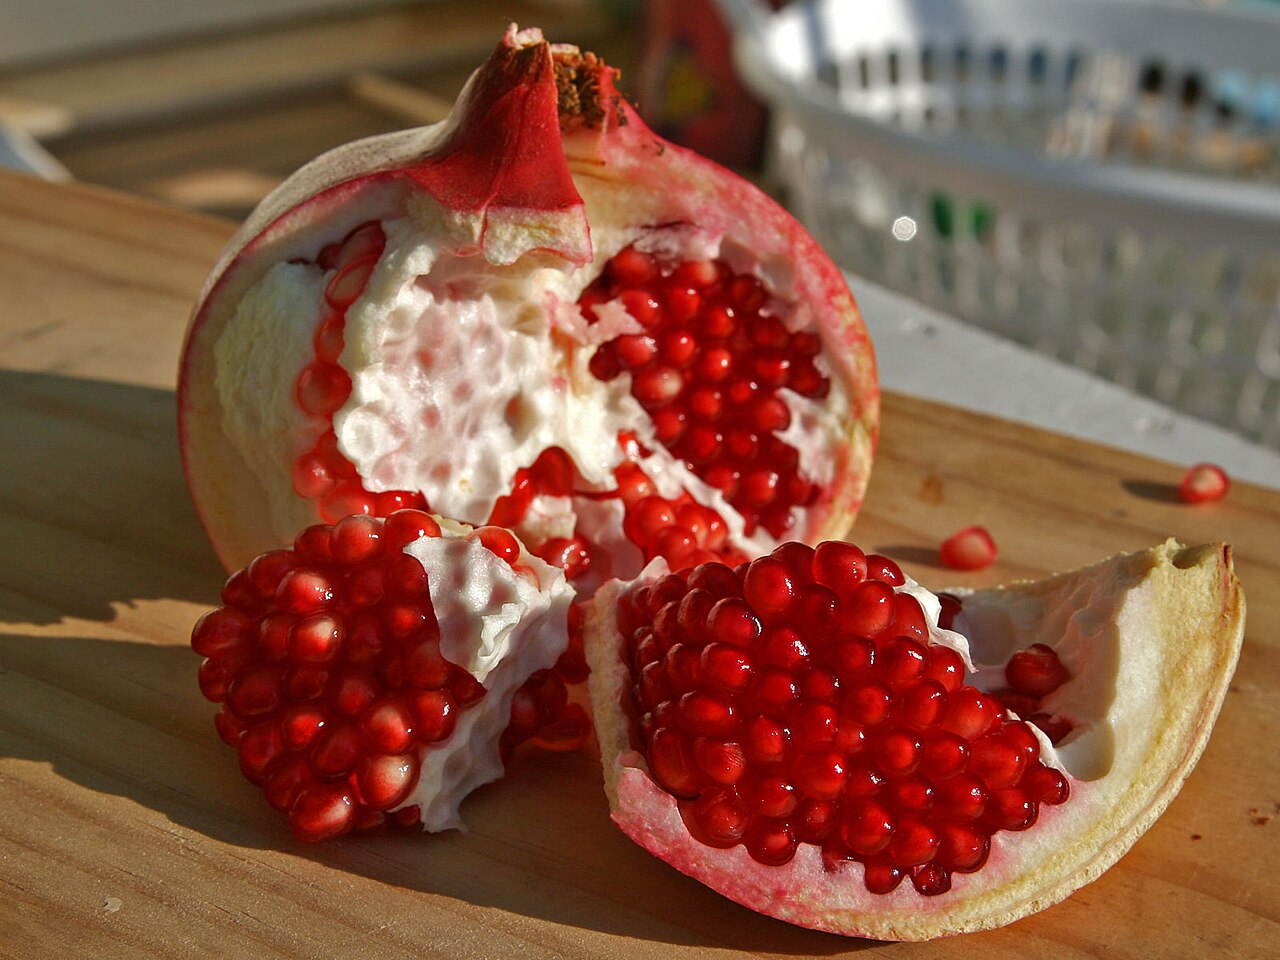
\includegraphics[width=\linewidth]{src_pomegranate.jpg}\\[2pt]
      {\scriptsize 2,000 of these - and that is all you get.}
    \end{center}
  \end{columns}
\end{frame}

\begin{frame}{Outline}
  \tableofcontents
\end{frame}

% ================================================================
\section{Transfer learning}

\begin{frame}[plain]
  \vfill
  \begin{center}
    {\Large\color{popblue}\textbf{Reuse features, not just architectures}}\\[0.9em]
    \begin{minipage}{0.82\textwidth}\centering\small
      Somebody already trained a net on 1.2 million images. Most of what it learned is
      about \emph{seeing}, not about their classes.
    \end{minipage}
  \end{center}
  \vfill
\end{frame}

\begin{frame}{Why transfer works}
  \begin{columns}[T]
    \column{0.48\textwidth}
    [48]: conv layers learn a \textbf{feature hierarchy} - edges $\to$ textures $\to$
    parts $\to$ objects.
    \vskip 6pt
    [49]: a pretrained net's conv1 filters \emph{are} the kernel zoo - edge and color
    detectors nobody designed.
    \vskip 6pt
    Edges and textures are the \textbf{same} for pomegranates, pets, and X-rays. Only the
    late, task-specific layers need \emph{your} data.
    \vskip 6pt
    \fcolorbox{armblue}{armblue!8}{\parbox{0.95\linewidth}{\small
      A pretrained network's conv layers are a general-purpose \textbf{visual feature
      extractor}. The hierarchy is the reusable asset.}}
    \column{0.52\textwidth}
    \begin{center}
      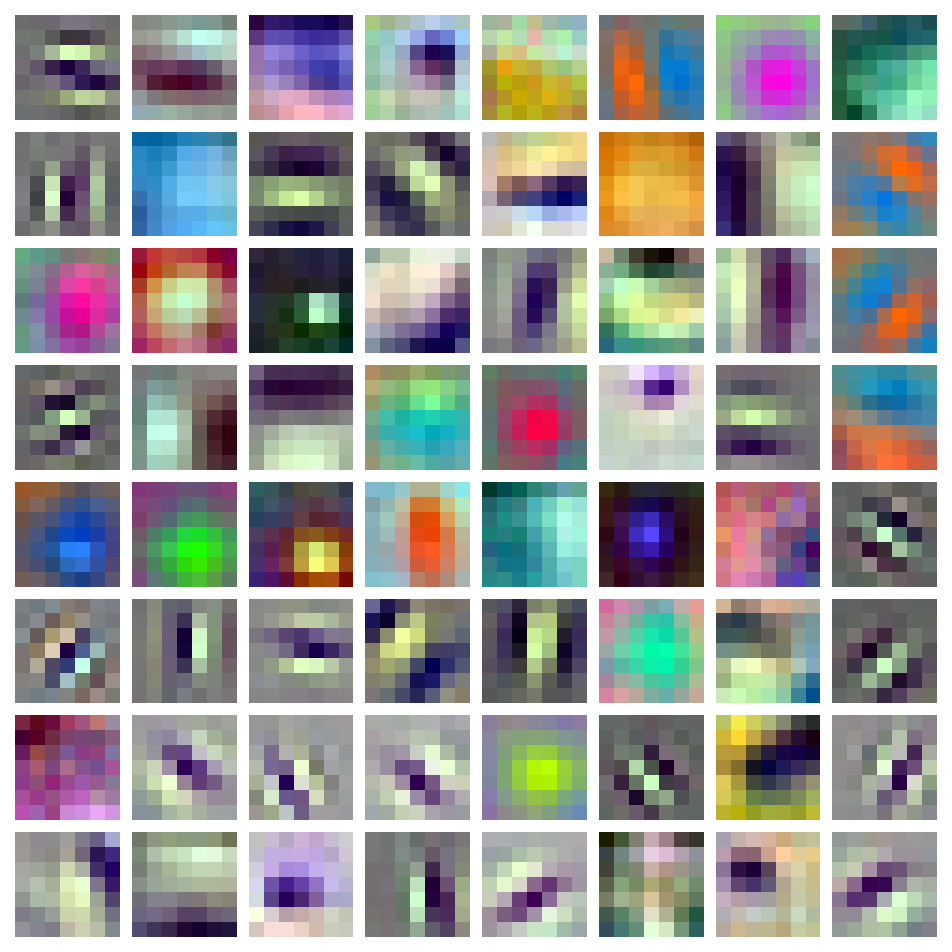
\includegraphics[width=0.72\linewidth]{pretrained_filters.pdf}\\[2pt]
      {\scriptsize The [49] payoff figure: learned on ImageNet, useful everywhere.}
    \end{center}
  \end{columns}
\end{frame}

% 2026-10-14 addition (instructor: "show the architecture at least once so the blocks make
% sense", "explain why the word trunk"). Figure from py_src/resnet18_arch.py: shapes traced through
% torchvision's resnet18 with forward hooks and asserted (56x56x64, 56x56x64, 28x28x128, 14x14x256,
% 7x7x512, avgpool 512, fc 3); the script also asserts 18 weight layers (conv1 + 16 3x3 convs + fc;
% the three 1x1 shortcut convs are not counted, as in He et al. 2015).
\begin{frame}{ResNet-18: a trunk and a head}
  \vskip -4pt
  {\centering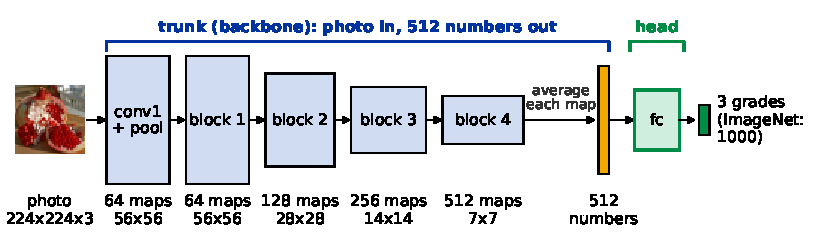
\includegraphics[width=0.9\linewidth]{resnet18_arch.pdf}\par}
  \vskip -2pt
  \begin{columns}[T]
    \column{0.53\textwidth}
    \small
    From block 2 on, each block \textbf{halves} the height and width and \textbf{doubles} the
    channels. Inside: two residual units of two $3\times3$ convs ([49]).
    \vskip 3pt
    \textbf{Where 512 comes from:} block 4 ends with 512 maps of $7\times7$; global average
    pooling ([49]) turns each map into one number. Those \textbf{512 numbers} are all the head
    ever sees.
    \column{0.45\textwidth}
    \fcolorbox{armblue}{armblue!8}{\parbox{0.95\linewidth}{\small
      \textbf{Why "trunk"?} Body words: the \textbf{head} sits on top and makes the call; the
      \textbf{trunk} (torso) carries almost all the weights. Keep the trunk, swap the head.
      Most papers say \textbf{backbone} - same part; [51] uses that word.}}
  \end{columns}
  \vskip 2pt
  {\scriptsize\color{gray} 18 $=$ conv1 $+$ 16 convs in the blocks $+$ fc. PyTorch names:
  \texttt{conv1}, \texttt{layer1}-\texttt{layer4}, \texttt{avgpool}, \texttt{fc}.}
\end{frame}

\begin{frame}{Two recipes}
  \textbf{(Click to unfreeze.)}
  \vskip 4pt
  \begin{center}
    \only<1>{\resizebox{0.97\textwidth}{!}{\trunkrow{frzcol}{frzcol}{frzcol}{frzcol}{frzcol}{trncol}}}%
    \only<2>{\resizebox{0.97\textwidth}{!}{\trunkrow{frzcol}{frzcol}{frzcol}{frzcol}{trncol}{trncol}}}%
    \only<3>{\resizebox{0.97\textwidth}{!}{\trunkrow{frzcol}{frzcol}{trncol}{trncol}{trncol}{trncol}}}%
    \only<4>{\resizebox{0.97\textwidth}{!}{\trunkrow{trncol}{trncol}{trncol}{trncol}{trncol}{trncol}}}%
  \end{center}
  \vskip 2pt
  \parbox[t][1.05cm][t]{\textwidth}{\small
    \only<1>{\textbf{Recipe 1 - feature extraction.} Freeze the whole trunk; train only a
      new head. The trunk is a fixed feature extractor - tiny data suffices.}%
    \only<2>{\textbf{Recipe 2 - fine-tuning.} Start by unfreezing the \emph{top} block -
      the most task-specific features - with a \textbf{small} learning rate (LR).}%
    \only<3>{With more data, unfreeze deeper. Early layers stay frozen longest - their
      features are the most generic.}%
    \only<4>{With enough data, everything trains - still at a small LR. Better ceiling,
      more ways to overfit.}}
  \vskip 2pt
  \fcolorbox{armblue}{armblue!8}{\parbox{0.97\linewidth}{\small
      \textbf{Feature extraction} $=$ new head only, tiny data suffices.
      \textbf{Fine-tuning} $=$ also nudge the trunk - needs more data, buys a better
      ceiling.}}
\end{frame}

% 2026-10-13 addition: per-stage parameter counts from py_src/trainable_params.py (torchvision
% resnet18 architecture, 3-class head, asserted): conv1+bn1 9,536; layer1 147,968; layer2 525,568;
% layer3 2,099,712; layer4 8,393,728 (75.1%); fc 1,539; total 11,178,051 (= 11,689,512 - 513,000
% for the 1000-class head + 1,539).
\begin{frame}{How much does each recipe actually train?}
  \begin{columns}[T]
    \column{0.44\textwidth}
    \small
    \textbf{Predict:} Recipe 2 starts by unfreezing \emph{one} of the five stages - the top
    block. What share of the weights is that?
    \vskip 6pt
    \onslide<2->{%
    Count them (3-grade head; {\color{paramgreen}\textbf{green}} = what the first unfreeze
    trains):
    \begin{itemize}\setlength\itemsep{1pt}
      \item head only: $512 \cdot 3 + 3 = \mathbf{1{,}539}$ - 512 numbers in (block 4's
        maps, averaged), 3 grades out, plus 3 biases;
      \item $+$ block 4: \textbf{8.4M} - \textbf{75\%} of the net;
      \item everything: \textbf{11.2M} (11.7M minus ImageNet's 1000-class head).
    \end{itemize}}
    \column{0.54\textwidth}
    \onslide<2->{\vskip 2pt{\centering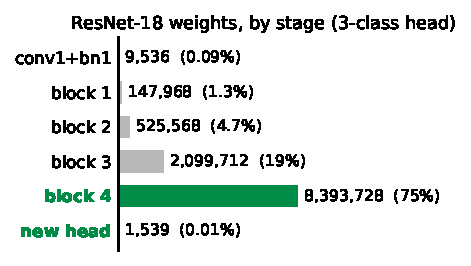
\includegraphics[width=\linewidth]{trainable_params.pdf}\par}}
  \end{columns}
  \vskip 4pt
  \onslide<2->{%
  \fcolorbox{armblue}{armblue!8}{\parbox{0.97\linewidth}{\small
    \textbf{Why the top is heavy:} channels double every stage and a $3\times3$ conv has
    $9 \cdot C_{\text{in}} \cdot C_{\text{out}}$ weights - double both, $4\times$ the weights.
    And Recipe 1 fits \textbf{1,539} numbers to \textbf{2,000} photos: [11]'s logistic
    regression on a $2{,}000 \times 512$ table - the cold open's problem, reversed.}}}
\end{frame}

\begin{frame}{Which recipe? Two questions decide}
  \begin{center}
    \begin{tikzpicture}[font=\small, >=Latex]
      % axes
      \draw[->, thick] (-0.1,0) -- (10.9,0);
      \draw[->, thick] (0,-0.1) -- (0,5.5);
      \node[anchor=north] at (2.6,-0.08) {\footnotesize small};
      \node[anchor=north] at (8.0,-0.08) {\footnotesize large};
      \node[anchor=north, gray] at (5.3,-0.5) {\textbf{your dataset size}};
      \node[rotate=90, gray] at (-1.2,2.65) {\textbf{domain similarity}};
      \node[anchor=east] at (-0.12,1.3) {\footnotesize far};
      \node[anchor=east] at (-0.12,4.0) {\footnotesize close};
      % cells
      \fill[paramgreen!14] (0.15,2.7) rectangle (5.25,5.25);
      \fill[paramgreen!24] (5.35,2.7) rectangle (10.6,5.25);
      \fill[armred!10]     (0.15,0.15) rectangle (5.25,2.6);
      \fill[armorange!16]  (5.35,0.15) rectangle (10.6,2.6);
      \node[align=center] at (2.7,4.15) {\textbf{feature extraction}\\[1pt]
        \footnotesize freeze the trunk,\\[-1pt] \footnotesize train the head};
      \node[align=center] at (7.95,4.15) {\textbf{fine-tune}\\[1pt]
        \footnotesize unfreeze some or all,\\[-1pt] \footnotesize small LR};
      \node[align=center] at (2.7,1.25) {\textbf{hardest case}\\[1pt]
        \footnotesize extract from \emph{earlier} layers\\[-1pt]
        \footnotesize + a simple head; get more data};
      \node[align=center] at (7.95,1.25) {\textbf{fine-tune everything}\\[1pt]
        \footnotesize pretrained init still helps};
      % running example marker
      \node[armred] at (1.35,3.25) {\textbullet};
      \node[armred, anchor=west] at (1.55,3.25) {\footnotesize the sorting line};
    \end{tikzpicture}
  \end{center}
\end{frame}

\begin{frame}{Fine-tuning in practice: you know all of this}
  \begin{itemize}
    \item \textbf{Small learning rate.} You start \emph{near a good minimum} - a big step
      jumps away from everything ImageNet taught the net ([44]'s learning-rate
      intuition).
    \item \textbf{Augmentation on.} Flips, crops, color jitter stretch 2,000 photos
      further ([43]).
    \item \textbf{Early stopping} on a validation split - the overfitting guardrail
      ([06], [43]).
    \item \textbf{Freeze first, unfreeze gradually} - the one genuinely new move today. Why
      it matters is the next slide.
  \end{itemize}
  \vskip 8pt
  \fcolorbox{paramgreen}{paramgreen!8}{\parbox{0.97\linewidth}{\small
      Fine-tuning is the [42]-[45] toolkit applied near a good minimum. Nothing new to
      learn - just new discipline.}}
\end{frame}

% 2026-10-13 addition (the deck said "freeze first" without the reason). Kumar, Raghunathan,
% Jones, Ma, Liang, "Fine-Tuning can Distort Pretrained Features and Underperform
% Out-of-Distribution", ICLR 2022 (oral), arXiv 2202.10054, abstract: over 10 datasets,
% fine-tuning is 2% higher ID but 7% lower OOD than linear probing; LP-FT is 1% better ID and
% 10% better OOD than full fine-tuning; mechanism = the lower layers change while the head is
% still being learned. Discriminative fine-tuning: Howard & Ruder, ULMFiT, ACL 2018.
\begin{frame}{Why freeze first? A random head bends the trunk}
  \small
  \textbf{Predict:} you unfreeze everything from step one, with a freshly initialized head.
  What do the first few hundred gradient steps do to the pretrained trunk?
  \vskip 4pt
  \onslide<2->{%
  \begin{itemize}\setlength\itemsep{2pt}
    \item The new head starts \textbf{random}: its outputs are noise, so the loss is large
      and so are its gradients.
    \item Backprop ([42]) carries those large, meaningless gradients \textbf{into the
      trunk}. The pretrained features get bent to suit a head that knows nothing yet.
    \item \textbf{Fix:} train the head alone first (Recipe 1 with a linear head - a
      \textbf{linear probe}), then unfreeze at a small learning rate: \textbf{linear
      probing, then fine-tuning} (\textbf{LP-FT}).
  \end{itemize}
  \vskip 2pt
  \fcolorbox{armblue}{armblue!8}{\parbox{0.97\linewidth}{\small
    \textbf{Measured} (Kumar et al., ICLR 2022, 10 datasets): plain fine-tuning beat the linear
    probe by 2\% on test photos like the training ones, but \textbf{lost by 7\%} on shifted
    ones - bent features generalize worse. LP-FT beat plain fine-tuning by 1\% and 10\%.}}
  \vskip 3pt
  \fcolorbox{armorange}{armorange!12}{\parbox{0.97\linewidth}{\small
    \textbf{One step further:} a learning rate per depth, largest for the head
    (\emph{discriminative fine-tuning}, Howard \& Ruder 2018) - generic features move least.}}}
\end{frame}

\begin{frame}{The BatchNorm gotcha}
  You froze the trunk: \texttt{requires\_grad = False} on every weight. Accuracy is
  still bad. Why?
  \vskip 6pt
  \begin{itemize}\small
    \item In \texttt{train()} mode BatchNorm (BN) normalizes each batch with \textbf{that
      batch's} mean and variance, and keeps updating \textbf{running averages} of them;
      \texttt{eval()} uses the running averages instead ([44] owns the formula).
    \item Those running averages are \textbf{not weights}: \texttt{requires\_grad =
      False} does not touch them, so they keep changing while "everything is frozen".
    \item Small batches from \emph{your} small dataset make the per-batch statistics noisy
      and drag the running averages away from the ImageNet values the frozen weights
      expect - accuracy drops \textbf{silently}.
  \end{itemize}
  \vskip 2pt
  {\small \textbf{How fast?} PyTorch updates
  $\text{running} \leftarrow 0.9\cdot\text{running} + 0.1\cdot\text{batch}$. Measured: a
  frozen BN layer in \texttt{train()} mode, stored mean $0$, fed 10 batches of mean $5$
  $\to$ running mean $3.26$ - already $65\%$ of the way ($1-0.9^{10}$) to your data.}
  \vskip 8pt
  \fcolorbox{armorange}{armorange!12}{\parbox{0.97\linewidth}{\small
      \textbf{Practical rule:} when the trunk is frozen, put its BN layers in
      \textbf{eval mode}. And whenever a "frozen" model underperforms - suspect the BN
      statistics first.}}
\end{frame}

\begin{frame}[fragile]{The canonical snippet}
  The whole of Recipe 1 - including the BatchNorm rule:
\begin{lstlisting}
from torchvision import models
import torch, torch.nn as nn

model = models.resnet18(weights="IMAGENET1K_V1")  # 11.7M trained weights
for p in model.parameters():
    p.requires_grad = False                       # freeze the trunk
model.fc = nn.Linear(model.fc.in_features, 3)     # new head: 3 grades
model.eval()                                      # BN: keep ImageNet stats
optimizer = torch.optim.SGD(model.fc.parameters(),
                            lr=0.001, momentum=0.9)
# then: the usual loop, minus model.train()
\end{lstlisting}
  \vskip 2pt
  \fcolorbox{paramgreen}{paramgreen!8}{\parbox{0.97\linewidth}{\small
      The new \texttt{fc} is created \emph{after} the freeze, so it trains by default -
      and it is the only thing the optimizer sees.}}
  \vskip 3pt
  \fcolorbox{armorange}{armorange!12}{\parbox{0.97\linewidth}{\small
      \textbf{\texttt{eval()} is not "no gradients".} It only switches BatchNorm (and dropout)
      to inference behaviour; gradients still reach \texttt{fc}. Gradients are a separate
      switch: \texttt{requires\_grad}.}}
\end{frame}

\begin{frame}{What transfer buys you}
  \begin{columns}[T]
    \column{0.40\textwidth}
    Same small dataset, three ways to train:
    \vskip 4pt
    \begin{itemize}
      \item \textbf{from scratch}: slow, plateaus low - 11.7M parameters memorize
        2,000 photos;
      \item \textbf{feature extraction}: fast and good;
      \item \textbf{fine-tune}: the best ceiling.
    \end{itemize}
    \vskip 6pt
    \fcolorbox{armblue}{armblue!8}{\parbox{0.95\linewidth}{\small
      \emph{Typical shapes}, not measurements. Gesture Snake measures two of them on your
      own photos: from scratch vs a frozen ResNet-18.}}
    \column{0.58\textwidth}
    \begin{center}
      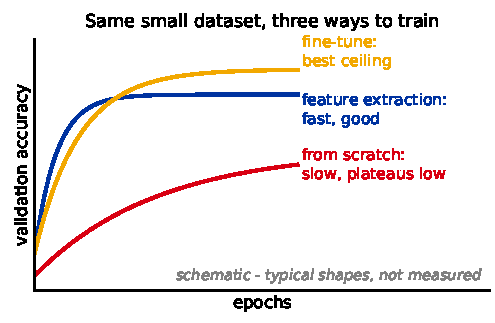
\includegraphics[width=\linewidth]{transfer_curves.pdf}
    \end{center}
  \end{columns}
\end{frame}

% 2026-10-13: third bullet from He, Girshick & Dollar, "Rethinking ImageNet Pre-training",
% ICCV 2019 (arXiv 1811.08883): random-init COCO detectors are "no worse than" ImageNet-pretrained
% ones given more iterations; pre-training "speeds up convergence" but "does not necessarily
% provide regularization or improve final target task accuracy". Input-contract box: torchvision
% 0.24 ResNet18_Weights.IMAGENET1K_V1.transforms() = resize 256, crop 224, bilinear, the
% ImageNet mean/std below (checked 2026-10-13).
\begin{frame}{When transfer fails - or stops mattering}
  \begin{itemize}\small
    \item \textbf{Domain too far.} Spectrograms, medical volumes, radar - ImageNet
      features stop being the right vocabulary. Unfreeze more, or rethink.
    \item \textbf{Bias mismatch.} ImageNet is object-centric daylight photography; data
      unlike that fights the pretrained assumptions.
    \item \textbf{Lots of data.} He, Girshick \& Doll\'ar (2019) trained COCO detectors from
      scratch and matched ImageNet-pretrained ones - given longer training. Pretraining
      bought \textbf{speed}, not a higher ceiling. 2,000 photos is nowhere near that regime.
  \end{itemize}
  \vskip 4pt
  \fcolorbox{armorange}{armorange!12}{\parbox{0.97\linewidth}{\small
      \textbf{Classic silent bugs - the input contract:} the pretrained net expects
      \textbf{its own} preprocessing, and quietly underperforms on anything else.
      \begin{itemize}\setlength\itemsep{0pt}
        \item ImageNet's mean $(0.485, 0.456, 0.406)$ and std $(0.229, 0.224, 0.225)$ -
          \emph{not} your dataset's;
        \item \texttt{cv2.imread} gives blue-green-red (\textbf{BGR}); the net wants RGB;
        \item simplest: \texttt{ResNet18\_Weights.IMAGENET1K\_V1.transforms()}.
      \end{itemize}}}
\end{frame}

% ================================================================
% 2026-10-14 (instructor: the jump from "when transfer fails" to the SSL frame was too quick):
% the three backbone frames became their own section with a transition slide.
\section{Bigger shoulders}

\begin{frame}[plain]
  \vfill
  \begin{center}
    {\Large\color{popblue}\textbf{Bigger shoulders, no labels}}\\[0.9em]
    \begin{minipage}{0.82\textwidth}\centering\small
      Everything so far stood on ImageNet: 1.2 million photos, each labeled by a person. The
      newest trunks learned from 400 million to 1.7 billion photos that nobody labeled by hand.
    \end{minipage}
  \end{center}
  \vfill
\end{frame}

% 2026-09-22 addition: the 2026 update to "whose features you borrow". DINOv3 facts from
% Meta's release blog (2025-08-14): 7B-param ViT, 1.7B unlabeled images, distilled ViT-B/L
% and ConvNeXt T/S/B/L variants, "state-of-the-art results ... without fine-tuning the
% backbone". Web-verified 2026-09-22.
% 2026-10-01 (l18_todo #1, "talk better about whose shoulders"): one frame became three, each
% with a diagram from py_src/backbone_diagrams.py. DINO: Caron et al. 2021 (self-distillation;
% the teacher is a slowly updated - moving-average - copy of the student; centering prevents
% collapse). CLIP: Radford et al. 2021, 400M image-text pairs, zero-shot ImageNet "matches the
% accuracy of the original ResNet-50". Web-checked 2026-10-01.
\begin{frame}{Shoulders without labels: self-supervised learning}
  \small
  Labels are the expensive part. Can a network learn to see from \textbf{photos alone}?
  \vskip 2pt
  \begin{center}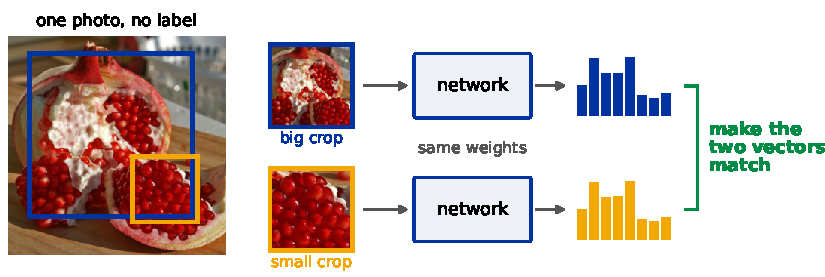
\includegraphics[width=4.15in]{ssl_crops.pdf}\end{center}
  \vskip 2pt
  \begin{columns}[T]
    \column{0.5\textwidth}
    \fcolorbox{armblue}{armblue!8}{\parbox{0.95\linewidth}{\scriptsize
      \textbf{Why it learns content:} a wide view and a close-up of the arils look very
      different pixel by pixel, but show the same thing. Matching vectors are only possible if
      they encode \emph{what} is there.}}
    \column{0.48\textwidth}
    \fcolorbox{armorange}{armorange!12}{\parbox{0.95\linewidth}{\scriptsize
      \textbf{The catch:} "the same vector for every photo" matches perfectly too. DINO avoids
      that collapse with a slowly updated "teacher" copy of the network and by centering its
      outputs.}}
  \end{columns}
  \vskip 3pt
  {\footnotesize Meta's \textbf{DINOv3} (2025): a 7-billion-parameter vision transformer
  trained this way on 1.7 billion unlabeled photos, built to be used \textbf{frozen} - and
  distilled into laptop-sized versions, including ConvNeXt CNNs ([49]).}
\end{frame}

\begin{frame}{Shoulders with words: CLIP}
  \small
  OpenAI's \textbf{CLIP} (2021) learned from \textbf{400 million image-caption pairs} from the
  web - nobody labelled them; the captions came for free.
  \vskip 2pt
  \begin{center}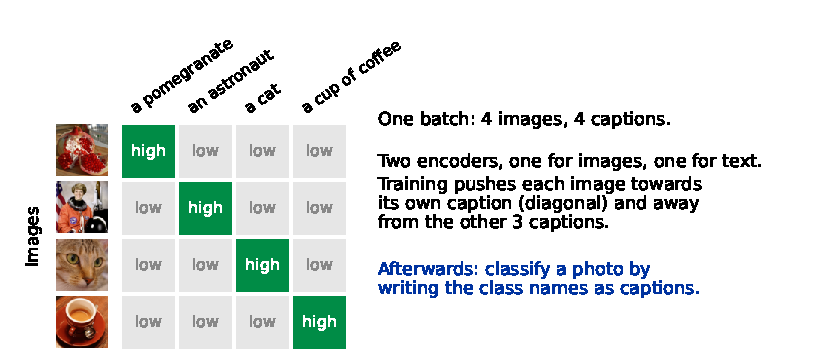
\includegraphics[width=4.1in]{clip_matrix.pdf}\end{center}
  \vskip 2pt
  \fcolorbox{armblue}{armblue!8}{\parbox{0.97\linewidth}{\small
    \textbf{Zero-shot:} embed "a photo of a pomegranate", "a photo of an apple", ..., and pick
    the caption closest to the photo. With no ImageNet training at all, CLIP matched the
    original ResNet-50 on ImageNet.}}
\end{frame}

\begin{frame}{2026: whose shoulders you stand on}
  Same two recipes - but the trunk is increasingly \textbf{not} an ImageNet classifier: it is a
  self-supervised (DINOv3) or image-text (CLIP) backbone.
  \vskip 6pt
  \begin{itemize}
    \item The \textbf{linear probe} from the LP-FT slide - freeze the trunk, fit one linear
      layer (logistic regression, [11]) on its features - is how these backbones are graded:
      the better the frozen features, the better a plain linear model does on top.
    \item The Gesture Snake practical does exactly this with a frozen ResNet-18.
  \end{itemize}
  \vskip 6pt
  \fcolorbox{paramgreen}{paramgreen!8}{\parbox{0.97\linewidth}{\small
    The sorting line's first try in 2026: frozen DINOv3 or CLIP features + a linear head.
    Fine-tune only if that is not enough. Bigger shoulders, and nobody had to label them.}}
\end{frame}

% ================================================================
\section{Seeing what the net sees}

\begin{frame}[plain]
  \vfill
  \begin{center}
    {\Large\color{popblue}\textbf{Trust, but verify}}\\[0.9em]
    \begin{minipage}{0.82\textwidth}\centering\small
      The fine-tuned model scores well. Before it grades a single truckload: \emph{what
      is it actually looking at?}
    \end{minipage}
  \end{center}
  \vfill
\end{frame}

\begin{frame}{Grad-CAM: where is the net looking?}
  \begin{columns}[T]
    \column{0.46\textwidth}
    \small
    Three steps, no new math:
    \vskip 3pt
    \begin{enumerate}
      \item<1-> Take the \textbf{last conv block's feature maps} - 512 coarse $7\times7$
        maps in ResNet-18: the most abstract "where" information left.
      \item<2-> \textbf{Weight each map by the gradient} of the class score with respect
        to it - one number per map: how much the score would rise if that map fired
        harder.
      \item<3-> \textbf{Sum, ReLU, upsample} - a heatmap of the evidence \emph{for} that
        class.
    \end{enumerate}
    \onslide<3->{\vskip 3pt
    \fcolorbox{armblue}{armblue!8}{\parbox{0.95\linewidth}{\small
      One forward, one backward, any trained CNN. Next: each step on our photo.}}}
    \column{0.54\textwidth}
    \begin{center}
      \only<1>{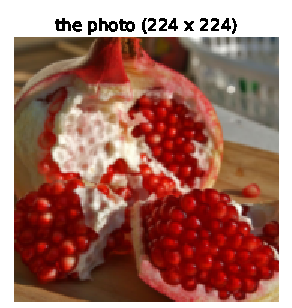
\includegraphics[width=1.8in]{gradcam_anim_0.pdf}}%
      \only<2>{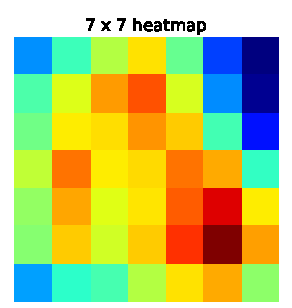
\includegraphics[width=1.8in]{gradcam_anim_1.pdf}}%
      \only<3>{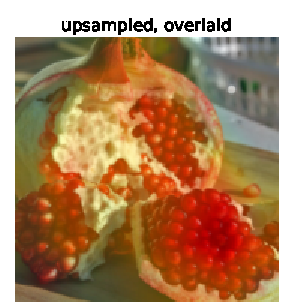
\includegraphics[width=1.8in]{gradcam_anim_2.pdf}}%
    \end{center}
  \end{columns}
  \vskip 2pt
  {\scriptsize\color{gray} Grad-CAM $=$ Gradient-weighted Class Activation Mapping
  (Selvaraju et al., ICCV 2017).}
\end{frame}

% 2026-10-01 (l18_todo #2: explain the gradient part; how do 512 7x7 maps become an image; show
% the gradients and the overlay; explain upsampling). Four step frames, figures from gradcam.py
% (one real ResNet-18 run on src_pomegranate.jpg). The script CHECKS the flat-gradient claim of
% step 2: every map's gradient is constant over its 49 cells and alpha_k = fc.weight[class,k]/49
% (max deviation 9e-10) - ResNet-18's GAP + linear head makes Grad-CAM equal CAM (Zhou et al. 2016).
\begin{frame}{Grad-CAM, step 1: the last feature maps}
  \small
  Our photo goes through ResNet-18. Its last conv block outputs \textbf{512 feature maps of
  $7\times7$}: each cell sits over a $32\times32$-pixel patch of the photo, and each map lights
  up where one high-level feature was found. Six of the 512:
  \vskip 4pt
  \begin{center}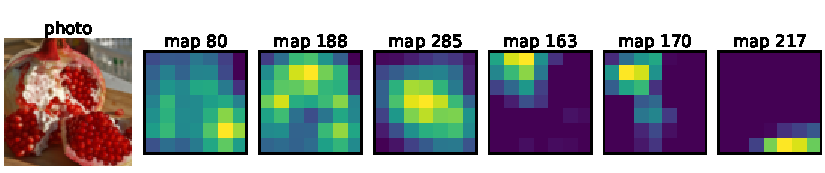
\includegraphics[width=5.5in]{gradcam_step1_maps.pdf}\end{center}
  \vskip 4pt
  \fcolorbox{armblue}{armblue!8}{\parbox{0.97\linewidth}{\small
    Each map says \emph{where}, none says \emph{what for}: some fire on the fruit, some on the
    background. Next: which maps matter for "pomegranate"?}}
\end{frame}

\begin{frame}{Grad-CAM, step 2: one weight per map, from the gradient}
  \small
  Ask backprop ([42]): if cell $(i,j)$ of map $k$ fired a little more, how much would the
  "pomegranate" score $y$ rise? That is $\partial y / \partial A^k_{ij}$. Average it over the 49
  cells: one weight per map, $\alpha_k = \frac{1}{49}\sum_{i,j} \partial y / \partial A^k_{ij}$.
  \vskip 2pt
  \begin{center}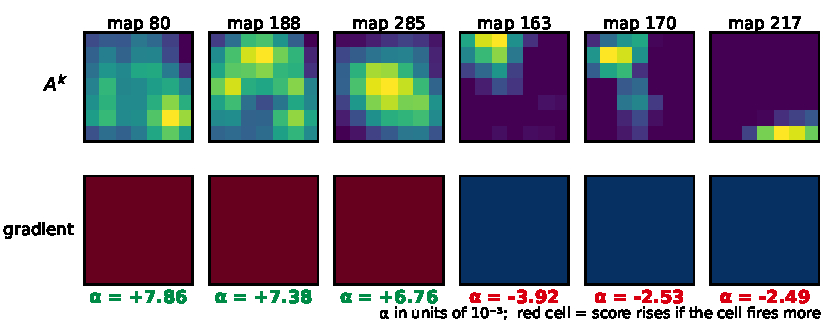
\includegraphics[width=4.4in]{gradcam_step2_grads.pdf}\end{center}
  \vskip 0pt
  \fcolorbox{armorange}{armorange!12}{\parbox{0.97\linewidth}{\scriptsize
    \textbf{Why is each gradient one flat colour?} ResNet-18 ends in a global average pool and
    one dense layer ([49]), so $y = \sum_k w_k \cdot \text{mean}(A^k)$ and $\partial y/\partial
    A^k_{ij} = w_k / 49$ in every cell: $\alpha_k$ is just the head's weight for map $k$. With
    a deeper head the gradient varies cell by cell; Grad-CAM works either way.}}
\end{frame}

\begin{frame}{Grad-CAM, step 3: weighted sum, then ReLU}
  \small
  Multiply each map by its weight and add all 512: maps that support "pomegranate" add, maps
  against it subtract. Then keep only the positive part:
  \[
    L = \text{ReLU}\Big(\sum_{k=1}^{512} \alpha_k A^k\Big) \qquad (7\times7)
  \]
  \vskip -2pt
  \begin{center}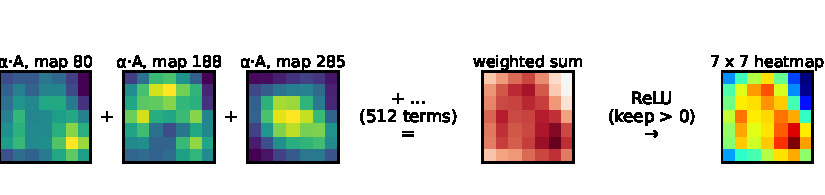
\includegraphics[width=5.5in]{gradcam_step3_sum.pdf}\end{center}
  \vskip 2pt
  \fcolorbox{armblue}{armblue!8}{\parbox{0.97\linewidth}{\small
    That is how 512 maps become \textbf{one} picture: a weighted vote, cell by cell. ReLU drops
    the evidence \emph{against} the class - we want what argued \emph{for} it.}}
\end{frame}

\begin{frame}{Grad-CAM, step 4: upsample to the photo}
  \small
  The heatmap is $7\times7$, the photo $224\times224$. \textbf{Upsampling} stretches the grid
  over the photo: each of the 49 values sits at the centre of its $32\times32$ patch, and
  every pixel in between gets a \textbf{blend of the four nearest values}, weighted by distance
  (bilinear interpolation).
  \vskip 2pt
  \begin{center}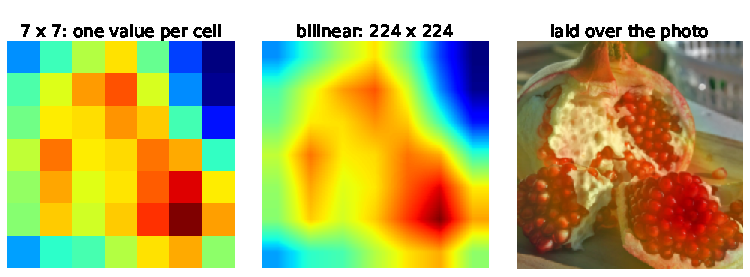
\includegraphics[width=5.0in]{gradcam_step4_upsample.pdf}\end{center}
  \vskip 2pt
  \fcolorbox{armblue}{armblue!8}{\parbox{0.97\linewidth}{\small
    Nothing new is learned here - the 49 numbers are only smoothed so they line up with the
    pixels. That is why Grad-CAM maps look blurry: their real resolution is $7\times7$.}}
\end{frame}

\begin{frame}{The verdict on our photo}
  \begin{columns}[T]
    \column{0.44\textwidth}
    \small
    No cherry-picking: an ImageNet ResNet-18, one forward and one backward, our photo.
    \vskip 4pt
    Top-1: \textbf{pomegranate}, $p = 0.99$. The evidence sits on the \textbf{fruit} -
    the aril clusters - not on the board or the basket.
    \vskip 4pt
    {\footnotesize Caveat: ImageNet \emph{has} a pomegranate class, so this is the easy
    case. The audit that matters is on a model trained on \emph{your} data - Gesture Snake
    runs it on your thumb model.}
    \vskip 4pt
    \fcolorbox{armblue}{armblue!8}{\parbox{0.95\linewidth}{\small
      The interpretability decks ([22]-[24]) asked which \textbf{features} matter -
      importance, SHAP. Grad-CAM asks which \textbf{pixels}. Same question, new
      coordinates.}}
    \column{0.55\textwidth}
    \begin{center}
      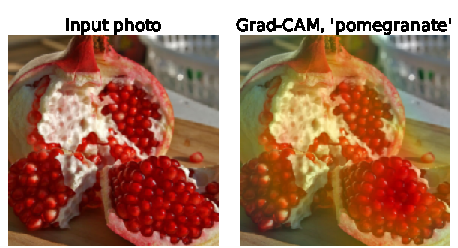
\includegraphics[width=\linewidth]{gradcam.pdf}
    \end{center}
  \end{columns}
\end{frame}

% 2026-10-13 addition: Grad-CAM's defining property (class-discriminative) and its limits.
% Figure = Selvaraju et al., arXiv 1610.02391v4, Fig. 1 panels (a), (c), (i) (VGG-16, 'tiger
% cat' and 'boxer'), cropped at 300 dpi -> fig/borrowed/gradcam_cat_dog.png. The paper's text:
% "the 'cat' explanation exclusively highlights the 'cat' regions but not 'dog' regions".
\begin{frame}{Ask about another class, get another map}
  {\centering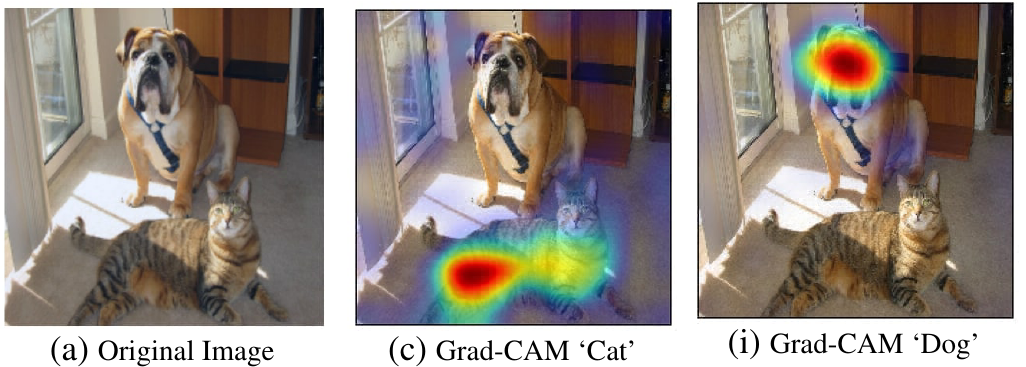
\includegraphics[width=3.1in]{gradcam_cat_dog.png}\par}
  \vskip 1pt
  {\scriptsize\color{gray}\hfill Selvaraju et al., ICCV 2017, Fig. 1 (VGG-16).}
  \vskip 1pt
  {\small The net outputs a score for \emph{every} class; step 2 differentiated the top one.
  \textbf{To ask about another class, backprop its score instead}:
  \texttt{model(x)[0, c].backward()} for class \texttt{c}. In our ResNet-18, $\alpha_k$ then
  comes from row \texttt{c} of the head: new weights, new map. Above: "cat" lights up the cat,
  "dog" the dog.}
  \vskip 4pt
  \begin{columns}[T]
    \column{0.49\textwidth}
    \fcolorbox{armblue}{armblue!8}{\parbox{0.95\linewidth}{\small
      \textbf{On the line:} on a fruit graded \emph{juice}, ask "why juice?" - the map
      should sit on the bruise, not on the belt.}}
    \column{0.49\textwidth}
    \fcolorbox{armorange}{armorange!12}{\parbox{0.95\linewidth}{\small
      \textbf{What it cannot tell you:} \emph{what} - a hot spot on the fruit cannot say
      colour, shape or sticker. And it sees on a $7\times7$ grid.}}
  \end{columns}
\end{frame}

\begin{frame}{Clever Hans, the vision edition}
  \begin{columns}[T]
    \column{0.48\textwidth}
    \begin{center}
      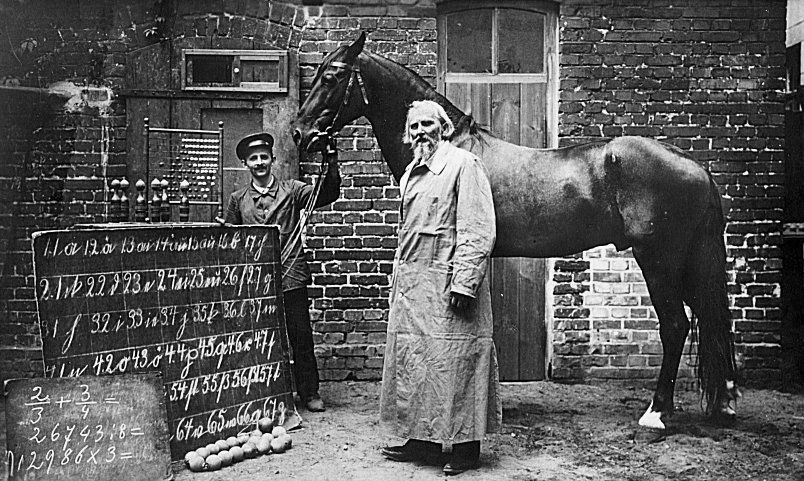
\includegraphics[width=0.62\linewidth]{clever_hans.jpg}
    \end{center}
    {\small Berlin, early 1900s: the horse \textbf{Clever Hans} "did arithmetic",
    tapping answers with a hoof. A 1907 investigation showed he was reading his
    questioner's \emph{unconscious posture}. Right answers, wrong reason.}
    \column{0.48\textwidth}
    \begin{center}
      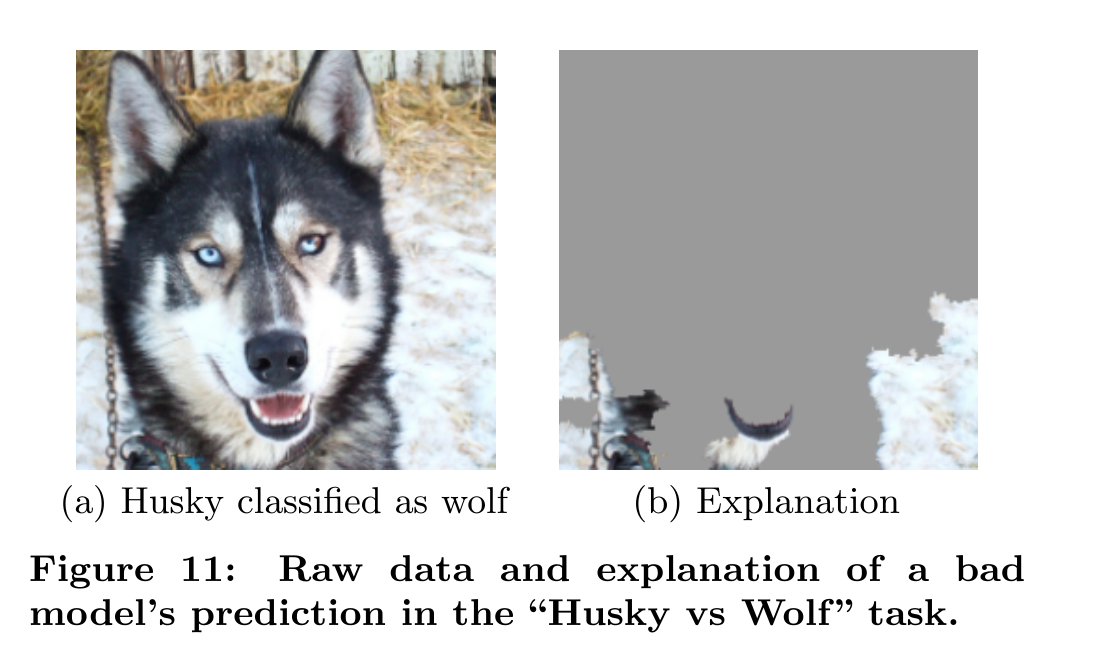
\includegraphics[width=0.62\linewidth]{wolf_husky_lime.png}
    \end{center}
    {\small A wolf-vs-husky classifier, trained where every wolf photo had \textbf{snow}
    in the background. It looked accurate - and was a \textbf{snow detector}
    (Ribeiro et al. 2016 - the LIME paper, [24]).}
  \end{columns}
  \vskip 2pt
  \fcolorbox{armred}{armred!8}{\parbox{0.97\linewidth}{\small
      On the sorting line: is the model grading the \textbf{fruit}, or the
      \textbf{conveyor belt} behind it? High accuracy is not right reasons. Grad-CAM is
      the five-minute check before you trust a model.}}
  \vskip 2pt
  {\scriptsize\color{gray} Ribeiro et al., "Why Should I Trust You?": Explaining the
  Predictions of Any Classifier, KDD 2016.}
\end{frame}

% ================================================================
\section{The economics of small data}

\begin{frame}[plain]
  \vfill
  \begin{center}
    {\Large\color{popblue}\textbf{The real budget is labels}}\\[0.9em]
    \begin{minipage}{0.82\textwidth}\centering\small
      GPUs are rented by the hour. Human attention is the expensive part.
    \end{minipage}
  \end{center}
  \vfill
\end{frame}

\begin{frame}{Somebody has to draw the boxes}
  \begin{itemize}
    \item Your 2,000 labeled photos meant somebody \textbf{looked at every single one} -
      hours of human attention, plus a second pass wherever labelers disagreed.
    \item Costs climb with detail: a class label is a \textbf{click}; a bounding box is a
      \textbf{drawing}; a per-pixel mask is a \textbf{tracing}. Each step up costs far
      more attention per image.
    \item Real projects spend their budget on \textbf{labels and label quality}, not on
      GPUs.
  \end{itemize}
  \vskip 8pt
  \fcolorbox{armblue}{armblue!8}{\parbox{0.97\linewidth}{\small
      Pretraining + transfer trade \textbf{your labels} for compute \textbf{somebody else
      already spent}. That is why transfer is the default - economically, not just
      statistically.}}
  \vskip 6pt
  {\small Hold that thought: [51]'s detection tasks need those \emph{boxes} - keep the
  price in mind.}
\end{frame}

% 2026-10-13 addition: the section promised economics and gave one frame of cost; this one gives
% the levers. Qualitative on purpose (the 2026-07 interview: zero invented numbers here).
\begin{frame}{Spending fewer labels}
  Transfer cut how \emph{many} labels you need. Four habits cut what each one costs:
  \vskip 4pt
  \begin{itemize}\setlength\itemsep{3pt}
    \item \textbf{Try zero labels first.} CLIP's zero-shot trick: "a photo of a bruised
      pomegranate" vs "a photo of a perfect pomegranate". Good enough? Done. If not, you
      learn \emph{where} it is confused.
    \item \textbf{Let a model draft, let people correct.} Accepting or fixing a pre-filled
      label is quicker than labeling from nothing - for boxes and masks even more ([51]).
    \item \textbf{Label what the model is unsure about}, not a random sample: a confident,
      correct prediction teaches it little (\emph{active learning}).
    \item \textbf{Consistency beats volume.} Two labelers who disagree on "market or juice"
      teach the model noise. Write the grading rule down; check agreement on a shared sample.
  \end{itemize}
  \vskip 6pt
  \fcolorbox{paramgreen}{paramgreen!8}{\parbox{0.97\linewidth}{\small
    The cheapest label is the one you never had to make - and the next cheapest is one a
    model drafted for you.}}
\end{frame}

% ================================================================
\section*{Recap}

\begin{frame}{Recap}
  \begin{itemize}
    \item With 2,000 photos, \textbf{never start from scratch} - reuse the feature
      hierarchy someone already paid to learn.
    \item A pretrained net $=$ \textbf{trunk} (photo $\to$ 512 numbers) $+$ \textbf{head}
      (512 numbers $\to$ classes). Transfer keeps the trunk and swaps the head.
    \item \textbf{Feature extraction}: train the head only (1,539 numbers).
      \textbf{Fine-tune}: head first, then unfreeze (LP-FT) at a small LR - and "just the top
      block" is 75\% of ResNet-18.
    \item Frozen trunk $\Rightarrow$ \textbf{BN to eval mode}; feed the net \textbf{its}
      preprocessing.
    \item \textbf{Grad-CAM}: per-class maps of \emph{where} (not \emph{what}) - the
      five-minute Clever Hans check.
    \item \textbf{Labels are the budget.} Transfer, zero-shot, model drafts and active
      learning all spend fewer of them.
  \end{itemize}
  \vskip 4pt
  \fcolorbox{paramgreen}{paramgreen!8}{\parbox{0.97\linewidth}{
      \textbf{Next:} the classifier is built and audited. But the belt camera sees
      \emph{ten} fruit at once - object detection and segmentation ([51]).}}
\end{frame}

\end{document}

% ================================================================
% Provenance:
%   Deck: L18 Transfer Learning and CNNs in Practice (12_cnn). Built 2026-07-14 from
%   50_transfer_learning_OUTLINE.md (approved, 2 interview rounds) + CNN_CHAPTER_PLAN.md.
%   (Chapter wrap-up 2026-10-17: the OUTLINE / QUESTIONS / NN_DECISIONS / HW1b_photoshop_PLAN
%   files named in these notes were deleted; `git show 1a62099:ml/12_cnn/<file>` recovers them.)
%   No LMU upstream - own material (transfer learning and Grad-CAM are not in the LMU
%   CNN decks). Facts sanity-checked against the web, not memory (2026-07-14):
%   - transfer recipe vs the official PyTorch transfer-learning tutorial
%     (docs.pytorch.org/tutorials/beginner/transfer_learning_tutorial.html): weights=
%     "IMAGENET1K_V1", fc replacement via fc.in_features, freeze via requires_grad=False,
%     optimizer on fc.parameters() only, SGD lr=0.001 momentum=0.9, ImageNet
%     normalization mean (0.485,0.456,0.406) / std (0.229,0.224,0.225).
%   - Grad-CAM vs Selvaraju et al., arXiv:1610.02391 (ICCV 2017): last conv layer's maps,
%     alpha_k = GAP of gradients of class score wrt A^k, weighted sum + ReLU, upsample.
%   - wolf-vs-husky: Ribeiro et al., KDD 2016 (arXiv:1602.04938), Figure 11 - classifier
%     trained so every wolf photo had snow; predicts from the snow.
%
%   Figures (py_src -> fig, ma venv):
%   - gradcam.pdf + gradcam_anim_0..2.pdf (gradcam.py): REAL run - torchvision resnet18
%     IMAGENET1K_V1 (11,689,512 params, hence "11.7M" on the slides), one forward+backward
%     on CPU, layer4 hooked, src_pomegranate.jpg. Actual top-1: 'pomegranate' p=0.995
%     (top-3: strawberry 0.004, trifle 0.001) - the p=0.99 on the verdict frame is the
%     measured value. Overlay uses per-pixel alpha (peak ~0.45, gamma 1.5) so the heatmap
%     reads as a spotlight over an already-red photo.
%   - transfer_curves.pdf (transfer_curves.py): SCHEMATIC - the HW3 notebook that will
%     produce real metrics does not exist yet, so the figure shows the three canonical
%     curve shapes with unlabeled axes and a printed "schematic - typical shapes, real
%     curves come with HW3" disclaimer. The script auto-switches to plotting measured
%     curves once py_src/data/hw3_metrics.csv appears (fails loudly on malformed files).
%   - pretrained_filters.pdf is L17's figure (generated by the L17 build), embedded here
%     as the "conv1 filters ARE the kernel zoo" callback - same file, not duplicated.
%   Borrowed (WEB-IMG, fig/borrowed/): wolf_husky_lime.png (the actual Figure 11 cropped
%   at 300 dpi from the arXiv LIME paper PDF), clever_hans.jpg (historic von Osten photo,
%   Wikimedia Commons "Osten und Hans.jpg").
%
%   Key decisions (details in 50_DECISIONS.md):
%   - 19 frames total vs the outline's ~16: the two-recipes frame split from the quadrant
%     frame (one idea per frame), and Grad-CAM split into idea (ANIM) + verdict (static).
%   - Mandatory ANIM = TikZ \only freeze/unfreeze trunk (4 clicks); optional Grad-CAM
%     ANIM also built (3 clicks: photo -> 7x7 map -> overlay).
%   - Interview-rejected extras honored: no live Colab demo, no in-class labeling
%     activity, no domain-gap failure demo. BN gotcha = claim + rule only, no evidence
%     figure. Labeling economics kept qualitative - zero invented numbers.
%
%   2026-09-22 pre-delivery pass (instructor away - autonomous): retired L15 callbacks
%   repointed to the delivered decks - LR intuition -> [44], augmentation + early stopping
%   -> [43], BatchNorm formula -> [44], "the L15 toolkit" -> [42]-[45]; "[05]" (a chapter
%   folder number, not a lecture) -> [22]-[24] for the interpretability decks and [24] for
%   LIME (24_shap_lime.tex carries the husky example). BatchNorm-gotcha mechanics corrected:
%   the old first bullet said BN "normalizes with running statistics", which is eval() mode;
%   train() normalizes with the current batch's statistics and only UPDATES the running
%   averages. NEW frame "2026: whose shoulders you stand on" (DINOv3 as a frozen
%   self-supervised backbone, CLIP, the term "linear probe"), facts from Meta's DINOv3 blog.
%
%   Same day, after a Sonnet student review of the rendered deck: the BatchNorm gotcha
%   gained a MEASURED drift number (frozen BN1d, train() mode, stored mean 0, 10 batches of
%   mean 5 -> running_mean 3.2566 = 5 * (1 - 0.9^10), PyTorch momentum 0.1, run 2026-09-23);
%   the Grad-CAM step 2 now says what the gradient weight means; the verdict frame admits
%   ImageNet has a pomegranate class (the easy, in-distribution case; the real audit is
%   HW3); the 2026 frame explains in one clause how label-free pretraining works (matching
%   features for two crops of one photo - the DINO family's idea, stated at intuition level).
%
%   2026-09-30 error fix (folder now ml/12_cnn): transition frame said "1.3 million images",
%   L17 says 1.2M three times (ILSVRC-2012 train = 1,281,167; the AlexNet paper writes "1.2
%   million"), so L18 now matches L17.
%
%   2026-10-01 round 2 (instructor's l18_todo.md):
%   - "2026: whose shoulders" became three frames: self-supervised learning (ssl_crops.pdf: two
%     crops, one network, matching vectors; why it learns content; the collapse catch), CLIP
%     (clip_matrix.pdf: the batch similarity table; zero-shot = captions as classes; matched the
%     original ResNet-50 on ImageNet), and the linear-probe frame with the sorting line's 2026 recipe.
%   - Grad-CAM: four new step frames after the overview, all figures from ONE real ResNet-18 run
%     (gradcam.py): (1) six of the 512 7x7 maps, (2) their gradients and alpha_k - every gradient
%     is flat because ResNet-18's head is GAP + linear, so alpha_k = w_k/49 (checked in the script,
%     max deviation 9e-10), (3) weighted sum + ReLU, (4) bilinear upsampling explained and shown.
%   - Figures redrawn at slide size: gradcam.pdf, gradcam_anim_0..2, transfer_curves.pdf.
%
%   2026-10-01 pass (instructor request "improve slides"): HW3 (Oxford-IIIT Pets) was never
%   built; both promises now point to the Gesture Snake practical (DECISIONS #58), which
%   measures a small CNN from scratch vs frozen ResNet-18 + linear head (Part 7) and runs
%   Grad-CAM on the student's own model (Part 5). transfer_curves.py's on-figure disclaimer
%   "real curves come with HW3" -> "not measured" (figure regenerated). Quadrant frame: the
%   rotated "domain similarity" label sat on top of "far" - moved left and centred. Grad-CAM
%   and LR spelled out.
%
%   2026-10-13 pedagogy + gaps pass (instructor: "improve them pedagogically, find important
%   gaps"); details and rejected alternatives in 50_DECISIONS.md #10-#16:
%   - FIX: the canonical snippet froze the trunk but ran "the usual loop" in train() mode - the
%     BatchNorm gotcha from the slide before. Now model.eval() + a box: eval() is not no_grad.
%   - NEW "How much does each recipe actually train?" (predict-first + by-hand counts,
%     trainable_params.py, counts asserted): head 1,539; layer4 8,393,728 = 75% of the 3-class
%     net (11,178,051); Recipe 1 = fewer parameters than photos = [11] on a 2,000 x 512 table.
%   - NEW "Why freeze first? A random head bends the trunk" (predict-first): the reason behind
%     "freeze first", LP-FT with Kumar et al. ICLR 2022's abstract numbers, discriminative LRs
%     (Howard & Ruder 2018). "Linear probe" is now defined here; the 2026 frame refers back.
%   - NEW "Two small-data traps" (predict-first, measured): random split vs burst split for
%     1-NN on pixels, 100.0% vs 43.2% (Gesture Snake Part 6, instructor's recordings), [06]
%     grouped-split callback; the label-changing flip (Part 3) and colour jitter on ripeness.
%   - "When transfer fails" -> "... or stops mattering": He, Girshick & Dollar 2019 (scratch
%     matches pretraining on COCO given longer training), input-contract box (ImageNet stats,
%     cv2 BGR, weights.transforms()).
%   - NEW "Ask about another class, get another map": Grad-CAM is class-discriminative (paper
%     Fig. 1 a/c/i, fig/borrowed/gradcam_cat_dog.png) + what it cannot tell you (what, 7x7).
%   - NEW "Spending fewer labels" (qualitative): zero-shot first, model drafts, active
%     learning, labeler consistency.
%   - Recap rewritten for the above; SSL frame figure 4.4in -> 4.15in (its last line sat in
%     the footer band).
%
%   2026-10-14 instructor review of that pass (50_DECISIONS.md #17-#21), 31 -> 32 frames:
%   - NEW "ResNet-18: a trunk and a head" (py_src/resnet18_arch.py, shapes traced + asserted, 18
%     weight layers asserted): stages, where the 512 comes from (GAP over block 4's 512 7x7
%     maps), why "trunk" (body words; "backbone" is the common synonym, [52] uses it). The
%     parameter-count frame's 512*3+3 bullet now names the 512.
%   - REMOVED "Two small-data traps" (instructor's call; the practical covers both) and its
%     recap bullet; a trunk + head recap bullet replaced it.
%   - NEW section "Bigger shoulders" + transition slide before the SSL / CLIP / 2026 frames.
%   - Grad-CAM "another class" frame says how: backprop that class's score,
%     model(x)[0, c].backward(); in ResNet-18 alpha_k comes from row c of fc.
%
%   Forward pointer: L19 Vision Tasks - detection (IoU/NMS, YOLO) + segmentation (U-Net),
%   chapter close. Practical after the chapter: Gesture Snake (ml/12_cnn/52_gesture_snake/).
%
%   2026-10-15: renumbered to the playlist after delivery (instructor: no practical between
%   [48] and transfer learning): [50] -> [49], [51] -> [50], [52] -> [51], the practical
%   [53] -> [52]; deck files renamed to match. Slide text uses the new labels; labels written in
%   this block before this date keep the old ones.
